\def\cleanbuild{}% all-black copy
\documentclass[pdflatex,sn-apa]{sn-jnl}% APA reference style (FODM)

\usepackage{graphicx}
\graphicspath{{figures/}{../figures/}}
\usepackage{amsmath,amssymb,amsfonts}
\usepackage{multirow}
\usepackage{booktabs}
\usepackage{xcolor}
\AtBeginDocument{\hypersetup{hidelinks}}
% Tables wider than the text block are scaled down to the text width (never enlarged). The class wraps
% every table in threeparttable, which cannot be boxed, so tables use the plain float and each tabular
% inside a table is set in a box first.
\newsavebox{\fitb}
\makeatletter
\AtBeginDocument{%
  \let\origtabular\tabular \let\endorigtabular\endtabular
  \def\fittabular{\setbox\fitb\hbox\bgroup\origtabular}%
  \def\endfittabular{\endorigtabular\egroup\ifdim\wd\fitb>\textwidth\resizebox{\textwidth}{!}{\usebox{\fitb}}\else\usebox{\fitb}\fi}%
  \renewenvironment{table}[1][htbp]{\begin{tableorg}[#1]\centering\tablebodyfont\let\tabular\fittabular\let\endtabular\endfittabular}{\end{tableorg}}}
\makeatother
% --- Change tracking (internal) ------------------------------------------
% \new{...} and \begin{newpart}...\end{newpart} mark revised text in blue.
% The submission copy is all black; remove the next line to see revisions in blue.
\newif\ifrevisionmarkup
\ifdefined\cleanbuild\revisionmarkupfalse\else\revisionmarkuptrue\fi
\definecolor{revblue}{RGB}{0,70,190}
\newcommand{\new}[1]{\ifrevisionmarkup\textcolor{revblue}{#1}\else#1\fi}
\newenvironment{newpart}{\ifrevisionmarkup\color{revblue}\fi}{}
% Numbered results: \stmt{counter}{label}{Name} prints `Name n' and sets the label.
\newcounter{lemma}\newcounter{definition}\newcounter{proposition}\newcounter{corollary}\newcounter{theorem}\newcounter{remark}
\newcommand{\stmt}[3]{\refstepcounter{#1}\label{#2}#3~\csname the#1\endcsname}
% Research questions: \rqdef{label} prints `RQn' and sets the label; \rqref{label} cites it.
\newcounter{rq}\newcommand{\rqdef}[1]{\refstepcounter{rq}\label{#1}RQ\therq}\newcommand{\rqref}[1]{RQ\ref{#1}}
% Notation macros: one definition per compound symbol.
\newcommand{\Rsys}{R_{\mathrm{sys}}}\newcommand{\Rtarget}{R_{\mathrm{target}}}
\newcommand{\kag}{k^{\alpha}(\gamma)}\newcommand{\WS}{\tilde{W}_S}\newcommand{\Zsuf}{Z^{\mathrm{suf}}}
\newcommand{\revtablecolor}{\ifrevisionmarkup\color{revblue}\fi}
% -----------------------------------------------------------------------
\usepackage[linesnumbered,ruled,vlined]{algorithm2e}
\SetAlFnt{\footnotesize}
% Float placement: keep tables, figures and the algorithm next to the text that cites them.
% [section] placeins flushes pending floats before each new section.
\usepackage[section]{placeins}
\renewcommand{\topfraction}{0.9}
\renewcommand{\bottomfraction}{0.8}
\renewcommand{\textfraction}{0.07}
\renewcommand{\floatpagefraction}{0.75}
\setcounter{topnumber}{3}
\setcounter{bottomnumber}{2}
\setcounter{totalnumber}{5}

\begin{document}

\title[Weighted $k$-out-of-$n$:G Systems under Dual Fuzziness]{Reliability Optimization of Weighted $k$-out-of-$n$:G Systems under Dual Fuzziness}

\author*[1]{\fnm{Kadir} \sur{Sar\i kaya}}\email{kadir.sarikaya@gop.edu.tr}
\affil*[1]{\orgdiv{Department of Industrial Engineering}, \orgname{Tokat Gaziosmanpa\c{s}a University}, \orgaddress{\city{Tokat}, \postcode{60150}, \country{T\"urkiye}}}

\abstract{\new{A weighted $k$-out-of-$n$:G system works when the total capacity of its working components reaches a demand threshold. In early-stage design, capacities and the threshold are often expert estimates. Weighted models with fuzzy or uncertain capacities keep the threshold crisp and evaluate given designs rather than optimize them. We propose a dual-fuzzy weighted $k$-out-of-$n$:G model in which component capacities and the demand threshold are triangular fuzzy numbers and success means that the fuzzy total capacity covers the fuzzy demand. A Hurwicz rule on $\alpha$-cuts, with a cut level and an optimism index, compares them; its range contains the crisp model, interval worst and best cases, and necessity-, possibility- and credibility-based chance constraints, making the attitude towards imprecision an explicit input. The weighted structure gives the main result: when all capacities share the same proportional spread, the two indices affect the design only through one integer threshold. One exact allocation problem per threshold, certified by a two-phase branch-and-bound algorithm, yields the optimal design for every index value. On an IEEE Reliability Test System and two literature-derived instances, a grid over the indices misses 29--48\% of the optimal designs, and crisp or one-sided models fail the target on up to half of the index range or overpay. The complete solution avoids both failures: a finite list of certified designs, each with its cost, guarantee and the index values where it is optimal, covers the whole index range and lets the decision maker choose a design instead of fixing the indices in advance.}}

\keywords{Weighted $k$-out-of-$n$:G system, Fuzzy reliability, Possibilistic chance constraint, Hurwicz criterion, Branch-and-bound, Power generation adequacy}

\maketitle

\section{Introduction}

\subsection{Background and Motivation}

The weighted $k$-out-of-$n$:G system (Wk/n:G) is a system of $n$ independent components in which each
component $i$ contributes an operational capacity $w_i > 0$ to the aggregate, and the system works if
and only if the total capacity of the working components meets or exceeds a prescribed threshold $k$:
\begin{equation*}
  \sum_{i=1}^{n} w_i \, s_i \;\geq\; k, \quad s_i \in \{0, 1\},
\end{equation*}
where $s_i = 1$ denotes that component $i$ is functioning. This formulation generalizes the classical
$k$-out-of-$n$:G model, in which every component contributes the same unit weight, to systems whose
components differ in performance, as is common in infrastructure such as generation fleets, pumping
stations and production lines with parallel units.

An efficient algorithm for evaluating the reliability of such systems was established by
\citet{WuChen1994}, whose $O(n \cdot k)$ recursion became the computational basis of later analytical
developments \citep{Kuo2007}. Building on this foundation, the scope of the Wk/n:G model was extended
along several dimensions. \new{\citet{Zhuang2022} evaluated the reliability and capacity of weighted
systems whose components have multiple performance levels and multiple states.} For such multi-state
systems the universal generating function (UGF) provides a general evaluation technique
\citep{Levitin2005}, and belief universal generating functions have been used to bring epistemic
uncertainty into static evaluations \citep{JaiswalNegiSingh2018}. \citet{DingZuoLisnianski2010} applied
the UGF approach to weighted multi-state systems and developed an approximation framework for
high-dimensional settings, later used for transmission-line networks \citep{SongEtAl2017}.
\citet{ZHANG2021107184} studied randomly weighted systems with heterogeneous components through
stochastic orders. \new{Related $k$-out-of-$n$ structures continue to be generalized, for example to
multi-state consecutive systems with sparse connections \citep{Gao2024sparse}.}

The model has also been extended to structural heterogeneity and to dynamic operating conditions.
\citet{EryilmazSarikaya2014} analyzed systems composed of two component types with different weight
distributions and derived exact reliability expressions. \citet{EryilmazBozbulut2014} developed a
time-dependent reliability framework for non-repairable multi-state Wk/n:G systems, and \citet{Xu2025} incorporated thermal balance into
dynamic reliability assessment for power-sensitive infrastructure. \new{\citet{Ozkut2025} studied
reliability analysis and optimization for Wk/n:G systems with several component types and crisp
capacities and thresholds.} \new{Maintenance studies derived inspection intervals for
load-sharing Wk/n:G systems \citep{Sharifi2023corr} and replacement strategies under shock models
\citep{LorvandKelkinnama2023}, \citet{Yang2022cbm} optimized condition-based maintenance for redundant
systems of arbitrary structure, and \citet{SinghSingh2025} studied cold-standby weighted systems with
multi-performance components.} Surveys of metaheuristic techniques for reliability
allocation document the use of the model across engineering domains \citep{Kuo2007,DeviGarg2023}.

\new{Despite these advances, most of the Wk/n:G literature treats the component weights $w_i$ as
\emph{crisp}, precisely known scalars, and the few studies with imprecise weights keep the success
threshold $k$ a fixed constant.} In many engineered systems neither assumption holds. Component
capacities change with mechanical wear, environmental conditions and manufacturing variability, and are
often known only through expert estimates. The threshold $k$ is rarely a physical constant; it is
usually a \emph{design judgement} derived from regulatory guidelines, expert consensus, safety standards
or demand forecasts. These sources carry \emph{epistemic uncertainty}, arising from incomplete
knowledge, rather than aleatory randomness, arising from variability in repeated trials.

\new{To make the consequences concrete, consider a regional grid operator that must deliver ``at least
$180$\,MW'' to downstream networks at peak demand. The $180$\,MW figure is a regulator's target, negotiated
from demand projections, seasonal load elasticity and measurement tolerance, and the available output of
each generating unit depends on ambient temperature and wear and is known mainly through expert
estimates.}

\new{A crisp formulation fixes both the capacities and the demand at nominal values. It thereby adopts a
risk posture without stating it:}
\begin{enumerate}
    \item \new{\emph{Exposure to shortfall.} A design that is feasible at nominal capacities may have
    zero necessity of meeting demand when the capacities fall within their plausible range.}
    \item \new{\emph{Hidden cost of conservatism.} Conversely, a requirement that demand be met with high
    necessity over the whole range of capacities may need considerably more redundancy,
    and capital, than the crisp design.}
\end{enumerate}
\new{A crisp formulation cannot distinguish these situations, because it never states how cautiously
capacity is compared with demand. The case study of Section~\ref{sec:rts_benchmark} is built on this setting.}

\subsection{Threshold Modeling Paradigms}

The reliability literature has acknowledged the limitations of a crisp, fixed threshold in several
ways, which lead to different structural formulations:

\begin{itemize}

\item \textbf{Multi-state $k$:} The threshold takes several discrete values across operating regimes, as
in \citet{Zhuang2022}. This relaxes the single-value assumption, but the threshold in each state remains
precisely specified.

\item \textbf{Phased-mission $k$:} In aerospace and military applications the success threshold changes
across temporally ordered mission phases. \citet{WangXingAmari2020} and \citet{WU2025110678} analyzed
phased-mission systems with decision diagrams and structural modeling techniques. Again, the threshold
of each phase is assumed crisp.

\item \textbf{Random $k$:} The threshold is a random variable with a specified probability distribution.
\citet{Eryilmaz2019} and \citet{Eryilmaz2021} formalized residual- and lost-capacity measures under
random thresholds, and \citet{Oszczypala2024} combined Markov-chain analysis with Monte Carlo simulation
for systems with probabilistically varying demand. Probabilistic threshold models need historical frequency data to characterize the distribution
of $k$. \new{In early-stage infrastructure design, capacity targets and derating bands come instead from
regulations, design codes and engineering consensus \citep{Helton2004}, and a probability distribution
then adds an assumption that the data do not support \citep{Zio2009}; possibility theory represents such
knowledge without a distributional assumption \citep{InuiguchiRamik2000,DuboisPrade2012}.}

\item \textbf{Fuzzy or uncertain $k$:} \new{Few studies treat the threshold itself as epistemically
imprecise; the closest studies make the component side imprecise instead. \citet{DingZuoLisnianski2010} represent the weights and state probabilities of
multi-state weighted systems by fuzzy numbers, obtained by clustering in order to approximate the
reliability of large systems; adequacy is evaluated against a prescribed demand through a
relative-cardinality measure, and no design problem is posed. Within Liu's uncertainty theory, \citet{Gao2018} and \citet{ShengKe2020}
analyze weighted $k$-out-of-$n$ systems whose weights and states are uncertain variables, and
\citet{WeiShiZhang2025a,WeiShiZhang2025b} extend this to two-stage systems with importance measures; in
all of these the threshold $k$ is a prescribed constant. \citet{Shi2021} treat a failure threshold as
uncertain, but for a degradation process rather than a weighted system, and without a design problem.}

\end{itemize}

\subsection{Fuzzy Modeling of Component Capacities}

Separately from threshold modeling, fuzzy set theory has been brought into component-level reliability
analysis. Fuzzy reliability concepts, founded on \citet{Zadeh1965} and \citet{DuboisPrade1988}, allow
reliability engineers to encode vague expert assessments as membership functions without presupposing a
probability distribution.

Within the reliability allocation problem, \citet{Chebouba2020} applied multi-objective genetic
algorithms to series--parallel systems with fuzzy component reliabilities. \citet{Ashraf2019} demonstrated type-2 fuzzy optimization on the
pharmaceutical plant benchmark. \citet{ChaubeSingh2016} and \citet{NegiSinghBisht2021} derived fuzzy
reliability expressions for higher-order weighted structures, and similar evaluations exist for linear
$m$-consecutive systems \citep{NegiSingh2019}. \new{\citet{ZhaoLiu2005} formulated standby redundancy
optimization under fuzzy component lifetimes.} Possibilistic reliability of standard $k$-out-of-$n$
systems was studied by \citet{HuangLiLiu2010}, and \citet{MANECKSHAW2026129956} proposed a
multi-objective allocation framework under epistemic uncertainty based on fuzzy possibility theory.

\new{As in the threshold paradigms above, component attributes are fuzzified here while the
\emph{failure boundary}, the threshold $k$, remains crisp. Once both sides of the success condition are fuzzy, the condition is
no longer an inequality between numbers, and a comparison rule must be chosen. A fuzzy capacity compared
with a crisp threshold has a conventional reading, so studies that fuzzify one side can leave the rule
implicit; studies that fuzzify both cannot. The rule determines which subsets count as successful and
therefore what the reported reliability means, yet it is rarely stated, and its relation to the standard
possibilistic measures is rarely examined.}

\new{Fuzzy redundancy-allocation models also fix one reading of the imprecise data in advance. Fuzzy
chance-constrained programming requires the constraints to hold with a given possibility
\citep{LiuIwamura1998}, credibility-based formulations use the self-dual credibility measure instead
\citep{Liu2002}, also on the cost and weight constraints of redundancy allocation \citep{HuangJiangYeh2020}, and interval models seek designs whose performance is robust over all
values in the intervals, for instance by minimizing the maximum regret \citep{FeizollahiModarres2012}. \citet{Ebrahimipur2011} optimize a multi-state weighted
$k$-out-of-$n$ allocation in which the reliability requirement and the cost budget are fuzzy goals with
tolerances, while the component capacities and the threshold remain crisp.}

\new{Table~\ref{tab:lit_position} compares this work with the closest related studies feature by
feature.}

\begin{table}[!htbp]
\centering
\caption{Comparison of related Wk/n:G modeling frameworks. ``Uncertain'' denotes Liu's uncertain measure rather than a possibility distribution; Gao et al. and Wei et al. represent component weights and states via uncertainty theory while keeping the demand threshold crisp. ``n/a'': no comparison between two imprecise quantities arises in the study. \new{Design task: ``Eval.'' computes the reliability (or a related measure) of a given design and optimizes no design; ``Heuristic opt.'' optimizes the design by a metaheuristic without a certificate of global optimality; ``Exact opt.'' optimizes the design and certifies the global optimum.}}
\label{tab:lit_position}
\footnotesize
\setlength{\tabcolsep}{3.5pt}
\begin{tabular}{lcccccccc}
\hline
\textbf{Feature} & \shortstack{Ding\\et al.\\(\citeyear{DingZuoLisnianski2010})} & \shortstack{Gao\\et al.\\(\citeyear{Gao2018})} & \shortstack{Negi\\et al.\\(\citeyear{NegiSinghBisht2021})} & \shortstack{Ashraf\\et al.\\(\citeyear{Ashraf2019})} & \shortstack{Eryilmaz\\\& Ucum\\(\citeyear{Eryilmaz2021})} & \shortstack{Maneckshaw\\et al.\\(\citeyear{MANECKSHAW2026129956})} & \shortstack{Wei\\et al.\\(\citeyear{WeiShiZhang2025a})} & \shortstack{\textbf{This}\\\textbf{paper}}\\
\hline
$\tilde{w}_i$ Fuzzy & Yes & Uncertain & No & No & No & No & Uncertain & \textbf{Yes}\\
$\tilde{k}$ Fuzzy & No & No & No & No & No & No & No & \textbf{Yes}\\
Design task & Eval. & Eval. & Eval. & \shortstack{Heuristic\\opt.} & Eval. & \shortstack{Heuristic\\opt.} & Eval. & \shortstack{\textbf{Exact}\\\textbf{opt.}}\\
Declared ordering & No & n/a & No & No & n/a & No & n/a & \textbf{Yes}\\
\hline
\end{tabular}
\end{table}

\subsection{Identified Research Gap and Research Questions}

\new{The review leaves three gaps. First, where capacities are treated as fuzzy or uncertain, the
threshold remains crisp \citep{DingZuoLisnianski2010,Gao2018,WeiShiZhang2025a}, while stochastic threshold
models require distributional knowledge that expert-driven design rarely has. Second, once both sides of
the success condition are imprecise, the comparison rule decides what the reported reliability means, yet
existing models either leave it implicit or fix one reading (a possibility, credibility or interval
criterion) before the design is chosen. Third, the weighted-system studies with imprecise weights evaluate
the reliability of a given design, and the studies in Table~\ref{tab:lit_position} that optimize a design
use heuristics without a certificate of global optimality. No study combines fuzzy capacities and a fuzzy
threshold with a declared comparison rule and an exact solver. This paper addresses these gaps through
three research questions:}
\begin{itemize}
  \item[\textbf{\rqdef{rq:rule}.}] \new{When component capacities and the threshold are both triangular fuzzy
  numbers, which comparison rule makes the success condition well defined, how does that rule
  relate to the necessity-, possibility- and credibility-based chance constraints, and which reliability measures does it induce?}
  \item[\textbf{\rqdef{rq:parametric}.}] \new{How do the cut level $\alpha$ and the optimism index $\gamma$ of the rule act
  on the optimal design and its cost, can the optimal design be determined for every value of
  $(\alpha,\gamma)$ rather than at sampled grid points, and what does a planner lose who samples the square
  on a grid or adopts a simpler model of the imprecision?}
  \item[\textbf{\rqdef{rq:solver}.}] \new{Can the resulting discrete redundancy-allocation problem be solved to
  certified global optimality at practical sizes, and what does certification change compared with a
  metaheuristic?}
\end{itemize}

\subsection{Research Contributions and Organization}

\begin{newpart}
The paper makes three contributions, one for each research question.
\begin{enumerate}
  \item \textbf{A dual-fuzzy weighted model with an explicit comparison rule (\rqref{rq:rule}).} We model both the component capacities and the demand threshold of a weighted $k$-out-of-$n$:G system as triangular fuzzy numbers, and success means that the fuzzy total capacity covers the fuzzy demand. The two are compared by a Hurwicz rule with two parameters, a cut level and an optimism index. We show that the usual readings of imprecise data (the crisp model, the interval worst and best cases, and necessity-, possibility- and credibility-based chance constraints) are special settings of these two parameters, so that they can be compared on the same instance with the same solver (Section~\ref{sec:theory}).
  \item \textbf{The optimal design for every parameter value (\rqref{rq:parametric}).} Because the system succeeds through the sum of its capacities, a common proportional spread scales that sum by one factor. We prove that the two parameters then affect the design only through one integer threshold, so that a small number of crisp problems, one per threshold, gives the optimal design everywhere instead of at the points of a grid (Section~\ref{sec:redundancy_framework}).
  \item \textbf{A certified exact solver (\rqref{rq:solver}).} A two-phase branch-and-bound algorithm returns the most reliable of the minimum-cost designs and certifies that it is globally optimal (Section~\ref{sec:solver}). It solves synthetic instances with up to $20$ subsystems, and a comparison with a genetic algorithm under the same computing budget shows when the certificate changes the selected design (Section~\ref{sec:results}).
\end{enumerate}
The evaluation uses a power-generation case study built from the IEEE Reliability Test System (RTS-79), a published benchmark that lists the capacities and forced outage rates of the generating units of a reference power system \citep{IEEERTS1979}, two instances derived from published allocation problems to check whether the findings recur, and a synthetic family for scalability. Against the complete solution we measure what a parameter grid and simpler models of the imprecision (the crisp model, one-sided fuzzy models and a probabilistic counterpart) lose, and we compare the exact solver with a genetic algorithm (Sections~\ref{sec:benchmarks} and~\ref{sec:results}).

Section~\ref{sec:theory} develops the dual-fuzzy model, the comparison rule and its possibilistic foundations (\rqref{rq:rule}). Section~\ref{sec:redundancy_framework} formulates the optimization model, proves the dimensional reduction (\rqref{rq:parametric}), presents the exact solver (\rqref{rq:solver}) and states the cost--necessity frontier problem. Section~\ref{sec:benchmarks} describes the instances, the protocol and the baselines, Section~\ref{sec:results} reports the results, Section~\ref{sec:discussion} discusses managerial implications, related frameworks and limitations, and Section~\ref{sec:conclusion} concludes.
\end{newpart}

\section{Dual-Fuzzy Model and Comparison Rule} \label{sec:theory}

\begin{table}[!t]
\caption{Nomenclature.}
\label{tab:nomenclature}
\footnotesize
\centering
\begin{tabular}{@{}ll@{}}
\toprule
\multicolumn{2}{@{}l}{\textbf{Indices and Sets}} \\
$n$ & Number of subsystems (components) \\
$i$ & Subsystem index, $i \in \{1, \dots, n\}$ \\
$j$ & Catalog design alternative index, $j \in M_i$ ($j=0$: no unit installed) \\
$M_i$ & Discrete catalog of available design alternatives for subsystem $i$ \\
$I(\mathbf{x})$ & Installed subsystems of design $\mathbf{x}$, $I(\mathbf{x}) = \{i : x_i \neq 0\}$ \\
$S$ & Subset of operational subsystems, $S \subseteq I(\mathbf{x})$ \\
$S^c$ & Subset of non-operational installed subsystems, $S^c = I(\mathbf{x}) \setminus S$ \\
$\mathbf{s}$ & Component state vector, $s_i = 1$ if component $i$ works and $0$ otherwise \\
\midrule
\multicolumn{2}{@{}l}{\textbf{Decision Variables and Physical Parameters}} \\
$x_i$ & Selected design alternative for subsystem $i$, $x_i \in M_i$ \\
$\mathbf{x}$ & System design configuration vector, $\mathbf{x} = (x_1, \dots, x_n)$ \\
$c_{i,j}, c_i(x_i)$ & Capital expenditure (cost) of choice $j$ in subsystem $i$ \\
$p_{i,j}$ & Intrinsic operational reliability of choice $j$ in subsystem $i$ \\
$\tilde{w}_i$ & Triangular fuzzy capacity weight of component $i$, $(w_{i,L}^0, w_i, w_{i,U}^0)$ \\
$W_S$, $\WS$ & Modal and fuzzy aggregate capacity of subset $S$, $\WS = \sum_{i \in S} \tilde{w}_i$ \\
$\delta_l, \delta_r$ & Common proportional left and right relative capacity spreads ($\delta$ when equal) \\
$\tilde{k}$ & Triangular fuzzy systemic demand threshold, $(k_1, k_2, k_3)$ \\
$\eta$ & Relative half-width of the demand forecast in the sensitivity study, $\tilde{k} = (k_2(1-\eta), k_2, k_2(1+\eta))$ \\
$\Rtarget$ & Prescribed minimum system reliability requirement \\
\midrule
\multicolumn{2}{@{}l}{\textbf{Possibilistic and Operational Metrics}} \\
$\alpha$ & Cut level of fuzzy sets, $\alpha \in [0, 1]$ \\
$\gamma$ & Hurwicz optimism-pessimism attitude index, $\gamma \in [0, 1]$ \\
$w_{i,L}^\alpha, w_{i,U}^\alpha$; $k_L^\alpha, k_U^\alpha$ & Lower and upper $\alpha$-cut endpoints of $\tilde{w}_i$ and $\tilde{k}$ \\
$\kag$, $w_i^\alpha(\gamma)$ & Hurwicz values of the threshold and of capacity $i$ (effective scalars), Eqs.~\eqref{eq:hurwicz_k} and~\eqref{eq:scalar_wi} \\
$m(\alpha,\gamma)$ & Capacity multiplier under common proportional spreads \\
$\kappa(\alpha,\gamma)$ & Effective continuous demand threshold, $\kappa = \kag / m(\alpha,\gamma)$ \\
$T$ & Effective integer capacity threshold, $T = \lceil \kappa(\alpha,\gamma) \rceil$ \\
$\gamma_T(\alpha)$ & Boundary of the region $\{\lceil\kappa\rceil = T\}$ in the policy square, Eq.~\eqref{eq:gamma_T} \\
$\lambda$ & Possibilistic chance-constraint confidence level, $\lambda \in (0, 1]$ \\
$\Pi, N, \mathrm{Cr}$ & Possibility, necessity, and credibility measures \\
$\Rsys^{\alpha,\gamma}(\mathbf{x})$ & Static (Hurwicz) reliability of design $\mathbf{x}$ under rule $(\alpha,\gamma)$, Eq.~\eqref{eq:static} \\
$\Pr(S \mid \mathbf{x})$ & Probability that exactly the components of $S$ work in design $\mathbf{x}$ \\
$R_N(\mathbf{x}), R_\Pi(\mathbf{x})$ & Expected necessity and possibility reliability of design $\mathbf{x}$, Eq.~\eqref{eq:rn_rpi_def} \\
$R_{\mathrm{modal}}(\mathbf{x})$ & Crisp reliability of design $\mathbf{x}$ at the modal demand $k_2$ \\
$R(\mathbf{x},T)$ & Crisp reliability of design $\mathbf{x}$ at the integer threshold $T$ \\
$D$, $\Theta$ & Random demand and common derating factor of the probabilistic counterpart \\
$\hat{T}$ & Random effective threshold of the probabilistic counterpart, $\hat{T} = \lceil D/\Theta \rceil$ \\
$R_{\mathrm{prob}}(\mathbf{x})$ & Reliability under the probabilistic counterpart, Eq.~\eqref{eq:rprob} \\
\midrule
\multicolumn{2}{@{}l}{\textbf{Optimization and Search}} \\
$Z(\mathbf{x})$ & Total capital cost of design $\mathbf{x}$, $Z(\mathbf{x}) = \sum_{i} c_i(x_i)$ \\
$Z^*$ & Minimum feasible cost (incumbent cost during the search) \\
$\mathcal{X}^*$ & Set of minimum-cost feasible designs, Eq.~\eqref{eq:opt_tiebreak} \\
$\bar{Z}$ & Capital budget \\
$r$ & Required expected necessity reliability on the cost--necessity frontier, $R_N(\mathbf{x}) \ge r$ \\
$Z_i^{\text{suf}}(q)$ & Minimum cost of subsystems $i+1,\dots,n$ that supply at least $q$ further capacity units \\
$K$ & Integer threshold of the search after scaling capacities to integers ($K = T$ under Theorem~\ref{thm:reduction}) \\
$\epsilon$ & Numerical tolerance on reliability comparisons, $\epsilon = 10^{-12}$ \\
$R_{\mathrm{ub}}$ & Optimistic upper bound on the reliability of any completion of a partial design (Theorem~\ref{thm:rel_bound}) \\
\midrule
\multicolumn{2}{@{}l}{\textbf{Abbreviations}} \\
FOR & Forced outage rate of a generating unit \\
IEEE RTS-79 & IEEE Reliability Test System (1979) \\
MTTF, MTTR & Mean time to failure, mean time to repair \\
MW & Megawatt \\
RQ & Research question \\
TFN & Triangular fuzzy number \\
UGF & Universal generating function \\
Wk/n:G & Weighted $k$-out-of-$n$:G (system) \\
\bottomrule
\end{tabular}
\end{table}

\subsection{Dual-Fuzzy Wk/n:G System Model}
The notation is summarized in Table~\ref{tab:nomenclature}. The weighted $k$-out-of-$n$:G (Wk/n:G) system consists of a set of independent components $C = \{1, 2, \dots, n\}$. The state of each component $i \in C$ is denoted by a binary indicator variable $s_i \in \{0, 1\}$, where $s_i = 1$ indicates that component $i$ is fully operational, and $s_i = 0$ indicates a failed state. Each component contributes a specific functional capacity, or weight, denoted by $w_i > 0$. The system state is defined by the state vector $\mathbf{s} = (s_1, s_2, \dots, s_n) \in \{0, 1\}^n$; the symbol $\mathbf{x}$ is reserved for the design vector of Section~\ref{sec:opt_model}.

The total capacity of the operational components is given by $W(\mathbf{s}) = \sum_{i=1}^n w_i s_i$. The classical system success function $\phi(\mathbf{s}): \{0,1\}^n \to \{0,1\}$ requires this aggregate capacity to meet or exceed a predefined system demand threshold $k$:
\begin{equation}
\phi(\mathbf{s}) = 
\begin{cases} 
1, & \text{if } W(\mathbf{s}) \geq k \\
0, & \text{otherwise}
\end{cases}
\end{equation}

\new{When both the component capacities and the demand threshold are subject to epistemic uncertainty, the dual-fuzzy model replaces the scalars $w_i$ and $k$ by fuzzy sets $\tilde{w}_i$ and $\tilde{k}$.} Let $S = \{i : s_i = 1\}$ denote the active subset of operational components for a given state $\mathbf{s}$. The aggregated fuzzy system capacity is derived via Zadeh's extension principle:
\begin{equation}
\WS = \sum_{i \in S} \tilde{w}_i
\end{equation}
\new{The success condition becomes a comparison of two fuzzy quantities,}
\begin{equation}
\WS \tilde{\geq} \tilde{k},
\end{equation}
\new{whose evaluation is defined in the next two subsections.}

\subsection{Mathematical Preliminaries: Possibilistic $\alpha$-Cuts}
Consider a general fuzzy set $\tilde{A}$ defined on the real line $\mathbb{R}$ with membership function $\mu_{\tilde{A}}(x): \mathbb{R} \to [0,1]$.
The crisp $\alpha$-cut at cut level $\alpha \in (0,1]$ is defined as the closed interval:
\begin{equation}
\tilde{A}^\alpha = \{x : \mu_{\tilde{A}}(x) \geq \alpha\} = [A_L^\alpha, A_U^\alpha],
\end{equation}
and for $\alpha=0$ it is defined as the topological closure of the support, $\tilde{A}^0 = \operatorname{cl}(\{x \in \mathbb{R} : \mu_{\tilde{A}}(x) > 0\}) = [A_L^0, A_U^0]$. \new{The cuts are nested: $\tilde{A}^{\alpha_2} \subseteq \tilde{A}^{\alpha_1}$ whenever $\alpha_1 < \alpha_2$.}

When specialized to Triangular Fuzzy Numbers (TFN), $\tilde{A} = (a_1, a_2, a_3)$, \new{the endpoints are linear in $\alpha$}:
\begin{equation}
[A_L^\alpha, A_U^\alpha] = [a_1 + \alpha(a_2 - a_1), a_3 - \alpha(a_3 - a_2)].
\label{eq:tfn_cut}
\end{equation}

\begin{newpart}
\subsection{Hurwicz Evaluation Rule and Crisp-Equivalence} \label{sec:hurwicz}
At cut level $\alpha$ the aggregate capacity of a subset $S$ is the interval $[W_{S,L}^\alpha, W_{S,U}^\alpha]$ and the threshold is the interval $[k_L^\alpha, k_U^\alpha]$. How two overlapping intervals are compared is a modeling assumption. We compare their Hurwicz values \citep{Hurwicz1951}, weighted by an optimism index $\gamma \in [0,1]$:
\begin{equation}
W_S^\alpha(\gamma) = \gamma W_{S,U}^\alpha + (1-\gamma) W_{S,L}^\alpha,
\label{eq:hurwicz_w}
\end{equation}
\begin{equation}
\kag = k_U^\alpha - \gamma (k_U^\alpha - k_L^\alpha).
\label{eq:hurwicz_k}
\end{equation}

\textbf{\stmt{definition}{def:hurwicz}{Definition} (Hurwicz Evaluation Rule under Cut Level $\alpha$ and Optimism $\gamma$).}
For $\alpha, \gamma \in [0,1]$, the fuzzy success condition $\WS \tilde{\geq} \tilde{k}$ holds at $(\alpha,\gamma)$ if and only if
\begin{equation}
W_S^\alpha(\gamma) \geq \kag.
\label{eq:success}
\end{equation}

At $\gamma = 0$ the rule compares the lowest capacity with the highest threshold, $W_{S,L}^\alpha \geq k_U^\alpha$ (pessimistic evaluation); at $\gamma = 1$ it compares the highest capacity with the lowest threshold, $W_{S,U}^\alpha \geq k_L^\alpha$ (optimistic evaluation). The convex weighting of interval endpoints follows \citet{Hurwicz1951} and its use in ranking fuzzy numbers under different risk attitudes \citep{CamposGonzalez1989,KimPark1990,LiouWang1992}. Under triangular data both sides of Equation~\eqref{eq:success} are affine in $\alpha$. The rule is defined on $\alpha$-cut intervals rather than on event spaces \citep{Yang2008}; Section~\ref{sec:family} shows that its columns $\gamma=0$ and $\gamma=1$ nevertheless coincide with necessity- and possibility-based chance constraints.

\textbf{\stmt{lemma}{lem:crisp_equiv}{Lemma} (Crisp-Equivalence of the Success Condition).}
\textit{For any active subset $S \subseteq \{1, \dots, n\}$, triangular fuzzy capacities $\tilde{w}_i = (w_{i,L}^0, w_i, w_{i,U}^0)$, triangular fuzzy demand $\tilde{k} = (k_1, k_2, k_3)$, and policy parameters $\alpha, \gamma \in [0,1]$, define the effective scalar component capacity:}
\begin{equation}
w_i^\alpha(\gamma) \;=\; \gamma \, w_{i,U}^\alpha + (1-\gamma) \, w_{i,L}^\alpha,
\label{eq:scalar_wi}
\end{equation}
\textit{and the effective scalar demand threshold $\kag$ as in Equation~\eqref{eq:hurwicz_k}. Then the fuzzy success condition of Equation~\eqref{eq:success} holds if and only if the sum of effective scalar capacities meets or exceeds the effective scalar threshold:}
\begin{equation}
\sum_{i \in S} w_i^\alpha(\gamma) \;\geq\; \kag.
\label{eq:crisp_equiv}
\end{equation}

\textit{Proof.} By Zadeh's extension principle, the aggregate fuzzy capacity is $\WS = \sum_{i \in S} \tilde{w}_i$. The $\alpha$-cut endpoints of a sum of fuzzy numbers are the sums of the component endpoints: $W_{S,L}^\alpha = \sum_{i \in S} w_{i,L}^\alpha$ and $W_{S,U}^\alpha = \sum_{i \in S} w_{i,U}^\alpha$. Substituting these into the Hurwicz combination of Equation~\eqref{eq:hurwicz_w} gives:
\begin{equation*}
W_S^\alpha(\gamma) \;=\; \gamma \sum_{i \in S} w_{i,U}^\alpha + (1-\gamma) \sum_{i \in S} w_{i,L}^\alpha \;=\; \sum_{i \in S} \left[\gamma \, w_{i,U}^\alpha + (1-\gamma) \, w_{i,L}^\alpha\right] \;=\; \sum_{i \in S} w_i^\alpha(\gamma).
\end{equation*}
Comparing $W_S^\alpha(\gamma)$ directly with $\kag$ establishes Equation~\eqref{eq:crisp_equiv}. $\square$

For any fixed pair $(\alpha,\gamma)$ and any capacity spreads, common or unit-specific, Lemma~\ref{lem:crisp_equiv} reduces the fuzzy success condition to a crisp weighted $k$-out-of-$n$:G condition with the scalar capacities $w_i^\alpha(\gamma)$ and the scalar threshold $\kag$. Dual fuzziness therefore defines a parameterized family of crisp Wk/n:G problems.
\end{newpart}

\begin{newpart}
\subsection{Possibilistic Foundations of the Rule} \label{sec:family}

Fuzzy quantities admit several ordering relations \citep{DuboisPrade1988,InuiguchiRamik2000}. This subsection shows that the standard possibilistic measures, possibility ($\Pi$), necessity ($N$) and credibility ($\mathrm{Cr}$), are linked to particular cells of the $(\alpha,\gamma)$ square, and Table~\ref{tab:nesting} collects the readings that the square contains.

Recall the two classical set-functions of \citet{DuboisPrade1988}. For triangular
$\tilde{A}=(a_1,a_2,a_3)$ and $\tilde{B}=(b_1,b_2,b_3)$, the possibility and necessity of the event
$\tilde{A}\ge\tilde{B}$ admit the closed forms
\begin{equation}
\begin{aligned}
\Pi(\tilde{A}\ge\tilde{B}) &=
\begin{cases}
1, & a_2 \ge b_2,\\[2pt]
\dfrac{a_3-b_1}{(a_3-a_2)+(b_2-b_1)}, & \text{otherwise,}
\end{cases}\\[6pt]
N(\tilde{A}\ge\tilde{B}) &=
\begin{cases}
0, & a_2 \le b_2,\\[2pt]
1-\dfrac{b_3-a_1}{(b_3-b_2)+(a_2-a_1)}, & \text{otherwise,}
\end{cases}
\end{aligned}
\end{equation}
both clipped to $[0,1]$. Possibility is the optimistic reading, which gives the event the benefit of
every doubt, and necessity the pessimistic one. Neither is self-dual, which is why
\citet{Liu2002} introduced the credibility measure
$\mathrm{Cr} = \tfrac{1}{2}\left(\Pi + N\right)$, which is self-dual. All three
are computed from the same triangular data as the Hurwicz values.

In this language a decision maker fixes a confidence level $\lambda$ instead of $(\alpha,\gamma)$ and
requires the success event to be necessary, or possible, at least to degree $\lambda$:
$N(\WS\ge\tilde{k}) \ge \lambda$ is a \emph{possibilistic chance constraint} in the sense of
\citet{InuiguchiRamik2000}. Proposition~\ref{prop:chance} maps such constraints onto cells of the policy square.

\textbf{\stmt{proposition}{prop:chance}{Proposition} (Chance-Constraint Correspondence).}
\textit{Let the capacities $\tilde{w}_i$ and the threshold $\tilde{k}$ be TFNs, and let the spreads that govern each branch be non-degenerate: $\sum_{i \in S}(w_i - w_{i,L}^0) + (k_3 - k_2) > 0$ for the necessity direction and $\sum_{i \in S}(w_{i,U}^0 - w_i) + (k_2 - k_1) > 0$ for the possibility direction. Then, for every confidence level $\lambda \in (0,1]$,}
\begin{equation}
N(\WS \ge \tilde{k}) \ge \lambda
\iff
W_S^{\,\alpha}(\gamma) \ge \kag
\quad\text{at }(\alpha,\gamma) = (1-\lambda,\,0),
\end{equation}
\begin{equation}
\Pi(\WS \ge \tilde{k}) \ge \lambda
\iff
W_S^{\,\alpha}(\gamma) \ge \kag
\quad\text{at }(\alpha,\gamma) = (\lambda,\,1).
\end{equation}

\textit{Proof.} Take the necessity branch with $a_2 > b_2$. Writing out
$N \ge \lambda$ using the closed form gives
$a_1 + (1-\lambda)(a_2-a_1) \ge b_3 - (1-\lambda)(b_3-b_2)$, whose two sides are precisely the lower
$\alpha$-cut endpoint of $\tilde{A}$ and the upper $\alpha$-cut endpoint of $\tilde{B}$ evaluated at
$\alpha = 1-\lambda$. By Equations~\eqref{eq:hurwicz_w} and~\eqref{eq:hurwicz_k} these are $W_S^{\alpha}(0)$ and $k^{\alpha}(0)$. When
$a_2 \le b_2$ the necessity is zero, so for $\lambda>0$ the constraint $N \ge \lambda$ fails, and under
the non-degenerate-spread assumption the pessimistic comparison fails as well. The restriction to
$\lambda>0$ is needed: at $\lambda=0$ the constraint $N \ge 0$ holds identically while the cell $(1,0)$
still demands $a_2 \ge b_2$, so the two are not equivalent there, and the possibility branch behaves in
the same way at $\lambda=0$. The possibility branch is symmetric, exchanging the roles of the
endpoints and reading $\alpha = \lambda$ at $\gamma=1$. $\square$

The two equivalences are the standard endpoint forms of necessity and possibility constraints
\citep{DuboisPrade1983,InuiguchiRamik2000}, and the conversion of possibilistic chance constraints into
crisp comparisons of interval endpoints is also used in chance-constrained formulations
\citep{Iskander2005,Maity2011}. Proposition~\ref{prop:chance} restates them in the notation of the
policy square, where they become its columns $\gamma=0$ and $\gamma=1$. As $\alpha$ sweeps $[0,1]$, the
column $\gamma=0$ enumerates every necessity-based chance constraint and the column $\gamma=1$ every
possibility-based one; a requirement such as ``demand met with necessity at least $0.7$'' is the cell
$(0.3,\,0)$. The interior columns $0<\gamma<1$ interpolate between the two attitudes and keep their
Hurwicz interpretation. Hurwicz evaluation and possibilistic chance-constrained programming are
therefore handled by one solver.

\textbf{\stmt{corollary}{cor:credibility}{Corollary} (Credibility Chance Constraints).} \textit{Under the assumptions of Proposition~\ref{prop:chance}, for every confidence level $\lambda \in (0,1]$,}
\begin{equation}
\mathrm{Cr}(\WS \ge \tilde{k}) \ge \lambda
\iff
W_S^{\,\alpha}(\gamma) \ge \kag
\quad\text{at }(\alpha,\gamma) =
\begin{cases}
(2\lambda,\,1), & \lambda \le 1/2,\\
(2-2\lambda,\,0), & \lambda > 1/2.
\end{cases}
\label{eq:credibility_cells}
\end{equation}

\textit{Proof.} For triangular numbers $N(\tilde{A}\ge\tilde{B})>0$ requires $a_2>b_2$, and then
$\Pi(\tilde{A}\ge\tilde{B})=1$. Let $\lambda>1/2$. If $N=0$, then $\mathrm{Cr}=\Pi/2\le 1/2<\lambda$; if
$N>0$, then $\mathrm{Cr}=(1+N)/2$. Hence $\mathrm{Cr}\ge\lambda$ if and only if $N\ge 2\lambda-1$. Let
$\lambda\le 1/2$. If $N>0$, then $\mathrm{Cr}\ge 1/2\ge\lambda$ and $\Pi=1\ge 2\lambda$; if $N=0$, then
$\mathrm{Cr}=\Pi/2$. Hence $\mathrm{Cr}\ge\lambda$ if and only if $\Pi\ge 2\lambda$. Since
$2\lambda-1\in(0,1]$ in the first case and $2\lambda\in(0,1]$ in the second, Proposition~\ref{prop:chance} maps the two
conditions to the cells $(2-2\lambda,0)$ and $(2\lambda,1)$. $\square$

The corollary follows from the definition of credibility \citep{Liu2002}; it states that credibility
chance constraints on the success condition are cells of the extreme columns of the square. The
expected credibility reliability, the probability-weighted average of $\mathrm{Cr}$ over the subsets,
is not a cell: like $R_N$ and $R_\Pi$ of Section~\ref{sec:decomposition}, it averages over the cut level. At $\lambda=1/2$ the cell is $(1,1)$, the
modal comparison $W_S\ge k_2$.

\textbf{\stmt{remark}{rem:central}{Remark} (The central column).} With symmetric spreads and a symmetric
threshold the central column $\gamma=1/2$ gives the modal comparison $W_S\ge k_2$, and hence the
credibility constraint at $\lambda=1/2$, at every $\alpha$. With an asymmetric threshold it does not: for
a crisp capacity $W_S=42$ and $\tilde{k}=(30,40,60)$ the cell $(0,1/2)$ requires
$W_S \ge k^0(1/2) = 45$, whereas $\mathrm{Cr}\ge 1/2$ requires only $W_S\ge 40$.

The closed forms of $\Pi$ and $N$, Proposition~\ref{prop:chance} and Corollary~\ref{cor:credibility} were
also checked numerically with asymmetric spreads and thresholds (Supplementary Material S2).

\begin{table}[!htbp]
\centering
\caption{Classical readings of the success condition $\WS\ge\tilde{k}$ as points of the policy
square (triangular capacities and threshold; Proposition~\ref{prop:chance} and Corollary~\ref{cor:credibility}, with $\lambda\in(0,1]$). The readings marked
``outside'' are not points of the square and are compared with it in Section~\ref{sec:baselines_res}
and Supplementary Material S4. \new{Supplementary Material S6 maps each reading to its threshold and optimal design on the IEEE RTS-79 fleet.}}
\label{tab:nesting}
\footnotesize
\begin{tabular}{lll}
\hline
Reading & Condition on subset $S$ & Location in the square\\
\hline
Crisp model at the modal values & $W_S \ge k_2$ & $\alpha=1$, any $\gamma$\\
Interval worst case on the supports & $W_{S,L}^{0} \ge k_U^{0}$ & $(0,0)$\\
Interval best case on the supports & $W_{S,U}^{0} \ge k_L^{0}$ & $(0,1)$\\
Necessity chance constraint & $N(\WS\ge\tilde{k}) \ge \lambda$ & $(1-\lambda,0)$\\
Possibility chance constraint & $\Pi(\WS\ge\tilde{k}) \ge \lambda$ & $(\lambda,1)$\\
Credibility chance constraint, $\lambda\le1/2$ & $\mathrm{Cr}(\WS\ge\tilde{k}) \ge \lambda$ & $(2\lambda,1)$\\
Credibility chance constraint, $\lambda>1/2$ & $\mathrm{Cr}(\WS\ge\tilde{k}) \ge \lambda$ & $(2-2\lambda,0)$\\
Expected necessity and possibility reliability & $R_N$, $R_\Pi$ (Eq.~\eqref{eq:rn_rpi_def}) & averages of the columns $\gamma=0$, $\gamma=1$\\
One-sided fuzzy models & $\tilde{w}_i$ or $\tilde{k}$ crisp & outside (other data)\\
Probabilistic counterpart & $\Pr\{\Theta W_S \ge D\}$ & outside\\
Liu's uncertainty theory & uncertain measure & outside (Supplementary S4)\\
\hline
\end{tabular}
\end{table}

\subsection{Reliability under Each Rule} \label{sec:decomposition}

The correspondences of Section~\ref{sec:family} concern the success condition of a single subset. A
reliability measure aggregates over subsets, and measures that agree on that condition can still assign
a design different reliabilities. Once a rule is fixed, the reliability of a design is the
probability of the subsets the rule accepts. For a design $\mathbf{x}$ (Section~\ref{sec:opt_model}) let $I(\mathbf{x}) = \{i : x_i \ne 0\}$ be the
set of subsystems in which a unit is installed, write $p_i = p_{i,x_i}$ and $\tilde{w}_i = \tilde{w}_{i,x_i}$
for the reliability and capacity of the installed unit, and let
$\Pr(S \mid \mathbf{x}) = \prod_{i \in S} p_i \prod_{l \in I(\mathbf{x}) \setminus S} (1-p_l)$ be the
probability that exactly the components of $S$ work. The static reliability of $\mathbf{x}$ at
$(\alpha,\gamma)$ is
\begin{equation}
\Rsys^{\alpha,\gamma}(\mathbf{x}) = \sum_{S \subseteq I(\mathbf{x}),\; \sum_{i \in S} w_i^\alpha(\gamma) \ge \kag} \Pr(S \mid \mathbf{x}).
\label{eq:static}
\end{equation}
The expected necessity and possibility reliabilities weight each subset by the necessity and the
possibility of its success instead:
\begin{equation}
R_N(\mathbf{x}) \;=\; \sum_{S \subseteq I(\mathbf{x})} \Pr(S \mid \mathbf{x}) \, N(\WS \ge \tilde{k}),
\qquad
R_\Pi(\mathbf{x}) \;=\; \sum_{S \subseteq I(\mathbf{x})} \Pr(S \mid \mathbf{x}) \, \Pi(\WS \ge \tilde{k}).
\label{eq:rn_rpi_def}
\end{equation}
The two families of reliability measures are linked through the extreme columns of the square.

\textbf{\stmt{proposition}{prop:decomposition}{Proposition} (Column Averages).} \textit{Under the
assumptions of Proposition~\ref{prop:chance}, for every design $\mathbf{x}$,}
\begin{equation}
R_{N}(\mathbf{x}) \;=\; \int_0^1 \Rsys^{\alpha,0}(\mathbf{x})\,d\alpha,
\qquad
R_{\Pi}(\mathbf{x}) \;=\; \int_0^1 \Rsys^{\alpha,1}(\mathbf{x})\,d\alpha .
\label{eq:decomposition}
\end{equation}

\textit{Proof.} Fix a subset $S$ and design $\mathbf{x}$. By Proposition~\ref{prop:chance}, for every $\alpha \in [0,1)$ the indicator of the cell
$(\alpha,0)$ accepting $S$ equals the indicator of $N(\tilde W_S \ge \tilde k) \ge 1-\alpha$; the single point $\alpha = 1$ does not affect the integral. Hence
$\int_0^1 \mathbf{1}\{S \text{ accepted at } (\alpha,0)\}\,d\alpha = N(\tilde W_S \ge \tilde k)$, which
is the layer-cake representation of a number in $[0,1]$. Multiplying by the probability $\Pr(S \mid \mathbf{x})$ and
summing over all subsets (both operations are linear and the sum is finite) yields the first identity in Equation~\eqref{eq:decomposition};
the second follows symmetrically at $\gamma=1$. $\square$

The expected necessity and possibility reliabilities are therefore the averages of the pessimistic and
optimistic columns over the cut level. A single cell of the necessity column also has a chance-constrained
reading: by Proposition~\ref{prop:chance}, the reliability constraint $\Rsys^{1-\lambda,0}(\mathbf{x}) \ge \Rtarget$ is equivalent to
\begin{equation}
\Pr \big\{ N(\WS \ge \tilde{k}) \ge \lambda \big\} \;\ge\; \Rtarget,
\end{equation}
that is, with probability at least $\Rtarget$ the available capacity clears the demand threshold with necessity at least $\lambda$.

\subsection{Monotonicity in the Cut Level} \label{sec:monotonicity}

\textbf{\stmt{proposition}{prop:alpha_monotone}{Proposition} (Conditional Monotonicity in $\alpha$).} \textit{For a fixed $\gamma$, suppose the evaluated subset capacity and threshold satisfy}
\begin{equation}
\frac{d}{d\alpha}W_S^\alpha(\gamma) \le 0, \qquad \frac{d}{d\alpha}\kag \ge 0
\end{equation}
\textit{for every subset $S$ of the installed components. Then the family $\mathcal{S}^{\alpha}$ of subsets accepted at $(\alpha,\gamma)$ is nested in $\alpha$, and}
\begin{equation}
\Rsys^{1,\gamma} \leq \Rsys^{\alpha,\gamma} \leq \Rsys^{0,\gamma}, \quad \alpha\in[0,1].
\end{equation}
\textit{Proof.} Under the stated derivative signs, increasing $\alpha$ cannot improve the success inequality $W_S^\alpha(\gamma) \ge \kag$ for any fixed subset $S$. Hence, if a subset is feasible at $\alpha_2$, it is also feasible at any $\alpha_1<\alpha_2$, implying $\mathcal{S}^{\alpha_2}\subseteq\mathcal{S}^{\alpha_1}$. Since $\Rsys^{\alpha,\gamma}$ sums nonnegative subset probabilities over these feasible sets, the ordering follows immediately. $\square$

\textbf{\stmt{remark}{rem:monotone_scope}{Remark} (Scope of the monotonicity).} The sign conditions of Proposition~\ref{prop:alpha_monotone} are sufficient, not universal. For a
component TFN $\tilde{w}_i = (w_{i,L}^0, w_i, w_{i,U}^0)$ with left and right spreads
$\Delta_i^{-} = w_i-w_{i,L}^0$ and $\Delta_i^{+} = w_{i,U}^0-w_i$, and a threshold with $\Delta_k^{-} = k_2-k_1$ and
$\Delta_k^{+} = k_3-k_2$,
\begin{equation}
\frac{d}{d\alpha}w_i^\alpha(\gamma) = (1-\gamma)\Delta_i^{-}-\gamma \Delta_i^{+},
\qquad
\frac{d}{d\alpha}\kag = \gamma \Delta_k^{-}-(1-\gamma)\Delta_k^{+},
\end{equation}
so, for spreads with $\Delta_i^{-}+\Delta_i^{+}>0$ and $\Delta_k^{-}+\Delta_k^{+}>0$ (a crisp quantity imposes no condition), the conditions hold if and only if $\gamma \ge \Delta_i^{-}/(\Delta_i^{-}+\Delta_i^{+})$ for every installed component and
$\gamma \ge \Delta_k^{+}/(\Delta_k^{-}+\Delta_k^{+})$. For symmetric data both reduce to $\gamma \ge 1/2$; a left-skewed TFN moves
the critical index towards $1$ (for $\Delta_i^{-}=10$, $\Delta_i^{+}=1$ the capacity derivative is positive for every
$\gamma<10/11$). For symmetric data and $\gamma<1/2$, which includes the necessity column, both signs are
reversed, and the same argument gives the reversed ordering
$\Rsys^{0,\gamma}\le \Rsys^{\alpha,\gamma}\le \Rsys^{1,\gamma}$; at $\gamma=1/2$ both derivatives
vanish and the reliability does not depend on $\alpha$. For general asymmetric data neither ordering need hold, and
the feasible-subset family need not be nested.

The exact solver does not rely on monotonicity: each $(\alpha,\gamma)$ cell is solved independently,
with bounds that are valid whether or not Proposition~\ref{prop:alpha_monotone} applies. Where monotonicity holds, it only
simplifies the interpretation of the results.
\end{newpart}

\section{Redundancy Allocation and Optimization Framework} \label{sec:redundancy_framework}

\subsection{Mathematical Optimization Model} \label{sec:opt_model}

In the discrete redundancy allocation problem, each subsystem $i \in \{1, \dots, n\}$ must be assigned exactly one design alternative from its discrete catalog $M_i$, which may contain a null option $j = 0$ (no unit installed, $w = 0$, $c = 0$). Each choice $j \in M_i$ specifies an operational capacity weight $\tilde{w}_{i,j}$, an intrinsic component reliability $p_{i,j}$, and a unit capital cost $c_{i,j}$.

Let the decision vector be $\mathbf{x} = (x_1, \dots, x_n)$, where $x_i \in M_i$ denotes the selected option for subsystem $i$. The primary objective in infrastructure redundancy planning is to minimize total capital expenditure required to guarantee that system reliability meets or exceeds a prescribed safety target $\Rtarget$ under the declared epistemic policy $(\alpha, \gamma)$. When multiple configurations achieve the minimum feasible cost, ties are broken in favor of the configuration delivering the highest reliability.

Formally, the exact optimization problem addressed across each $(\alpha, \gamma)$ policy cell is:
\begin{align}
\min_{\mathbf{x}} \quad & Z(\mathbf{x}) \;=\; \sum_{i=1}^{n} c_i(x_i) \label{eq:opt_cost} \\
\text{subject to} \quad & \Rsys^{\alpha,\gamma}(\mathbf{x}) \;\ge\; \Rtarget, \label{eq:opt_rel} \\
& x_i \in M_i, \quad \forall i \in \{1, \dots, n\},
\end{align}
governed by the secondary lexicographic tie-breaking criterion:
\begin{equation}
\max_{\mathbf{x} \in \mathcal{X}^*} \quad \Rsys^{\alpha,\gamma}(\mathbf{x}),
\label{eq:opt_tiebreak}
\end{equation}
where $\mathcal{X}^* = \arg\min \{Z(\mathbf{x}) : \Rsys^{\alpha,\gamma}(\mathbf{x}) \ge \Rtarget\}$ is the set of minimum-cost feasible designs.

\textbf{\stmt{remark}{rem:zimmermann}{Remark} (Relation to Zimmermann aggregation).} In flexible budgeting environments without a mandatory reliability threshold, a decision maker could alternatively model cost minimization and reliability maximization as conflicting fuzzy goals using Zimmermann's max--min aggregation $\max \mu_D = \min(\mu_{\text{Cost}}, \mu_{\text{Rel}})$ \new{\citep{Zimmermann2001}}. \new{When $\Rtarget$ is a contractual specification, that aggregation would add cost tolerance parameters that are not part of the problem data. The lexicographic formulation of Equations~\eqref{eq:opt_cost}--\eqref{eq:opt_tiebreak} uses only the problem data and admits a certificate of global optimality.}


\begin{newpart}
\subsection{Dimensional Reduction of the Policy Square} \label{sec:reduction}

The dual-fuzzy formulation asks for one optimization per point of the square
$(\alpha,\gamma) \in [0,1]^2$, and computational studies in fuzzy allocation therefore report results on
a coarse grid. Under the proportional spread model used in this paper, the square reduces to a single
parameter.

Assume, as in the base case of every instance of Section~\ref{sec:benchmarks}, that each capacity is fuzzified proportionally,
$\tilde{w}_i = \big(w_i(1-\delta_l),\, w_i,\, w_i(1+\delta_r)\big)$, with spread parameters
$\delta_l, \delta_r \in [0,1)$ that are the same for every component. By Zadeh's extension principle
the aggregate over any active subset $S$ inherits the same shape,
$\WS = \big(W_S(1-\delta_l),\, W_S,\, W_S(1+\delta_r)\big)$, where $W_S = \sum_{i \in S} w_i$
is the \emph{modal} total.

\textbf{\stmt{theorem}{thm:reduction}{Theorem} (Dimensional Reduction).}
\textit{Let the capacities be proportionally fuzzified with common spreads $\delta_l,\delta_r \in [0,1)$,
let the threshold $\tilde{k}$ be an arbitrary TFN, and let $\alpha,\gamma \in [0,1]$. Define the}
\emph{capacity multiplier}
\begin{equation}
m(\alpha,\gamma) \;=\; 1 - \delta_l(1-\alpha) + \gamma(\delta_l+\delta_r)(1-\alpha),
\label{eq:multiplier}
\end{equation}
\textit{which is strictly positive and independent of the subset $S$ and of the component index $i$. Then the
success condition of Equation~\eqref{eq:success} is equivalent to a comparison of the modal total against a single
scalar,}
\begin{equation}
W_S^{\alpha}(\gamma) \ge \kag
\iff
W_S \;\ge\; \kappa(\alpha,\gamma) \;=\; \frac{\kag}{m(\alpha,\gamma)} .
\label{eq:kappa}
\end{equation}

\textit{Proof.} With common proportional spreads every capacity is a scalar multiple of one common unit,
$\tilde{w}_i = w_i \cdot \tilde{u}$ with $\tilde{u} = (1-\delta_l,\,1,\,1+\delta_r)$. Scalar
multiplication distributes over the extension-principle sum \citep{DuboisPrade1978}, so
$\WS = W_S \cdot \tilde{u}$ and the aggregate $\alpha$-cut endpoints are
$W_{S,L}^{\alpha} = W_S\big(1-\delta_l(1-\alpha)\big)$ and
$W_{S,U}^{\alpha} = W_S\big(1+\delta_r(1-\alpha)\big)$. Substituting these into the Hurwicz
combination of Equation~\eqref{eq:hurwicz_w} and factoring $W_S$ gives $W_S^{\alpha}(\gamma) = W_S \cdot
m(\alpha,\gamma)$ with $m$ as in Equation~\eqref{eq:multiplier}. Since $\delta_l < 1$ and
$\gamma \ge 0$, we have $m > 0$, so dividing both sides of the success condition by $m$ preserves the
inequality. $\square$

Theorem~\ref{thm:reduction} uses the distributivity of scalar multiplication over fuzzy
addition \citep{DuboisPrade1978}, as do reductions of possibilistic constraints
\citep{InuiguchiRamik2000,Rommelfanger1996,CadenasVerdegay1997}. In a discrete multi-choice design
problem, $\lceil\kappa(\alpha,\gamma)\rceil$ takes finitely many values over the unit square. The square
therefore splits into finitely many regions with closed-form boundaries, and the parametric solution
over the whole square can be computed exactly, which extends parametric analysis
\citep{CarlssonKorhonen1986} to discrete multi-choice catalogs.

\textbf{\stmt{corollary}{cor:partition}{Corollary} (Closed-Form Partition Boundaries).}
\textit{For each integer threshold $T \in \mathbb{Z}^+$ and cut level $\alpha \in [0, 1)$, the boundary curve separating the region where $\kappa(\alpha,\gamma) \le T$ from $\kappa(\alpha,\gamma) > T$ in the $(\alpha,\gamma)$ policy square is given explicitly in closed form by:}
\begin{equation}
\gamma_T(\alpha) \;=\; \frac{k_U^\alpha - T\big(1 - \delta_l(1-\alpha)\big)}{(k_U^\alpha - k_L^\alpha) + T(\delta_l + \delta_r)(1-\alpha)},
\label{eq:gamma_T}
\end{equation}
\textit{where $k_L^\alpha = k_1 + \alpha(k_2 - k_1)$ and $k_U^\alpha = k_3 - \alpha(k_3 - k_2)$ denote the lower and upper $\alpha$-cut endpoints of the threshold $\tilde{k} = (k_1, k_2, k_3)$. Since $\kappa$ is decreasing in $\gamma$ for $\alpha<1$, the region on which $\lceil\kappa\rceil = T$ is $\{\gamma \in [0,1] : \gamma_T(\alpha) \le \gamma < \gamma_{T-1}(\alpha)\}$; when $\gamma_{T-1}(\alpha) > 1$ it contains $\gamma = 1$, and when $\gamma_T(\alpha) < 0$ it contains $\gamma = 0$.}

\textit{Proof.} Equating $\kappa(\alpha,\gamma) = T$ in Equation~\eqref{eq:kappa} gives $\kag = T \cdot m(\alpha,\gamma)$. Substituting $\kag = k_U^\alpha - \gamma(k_U^\alpha - k_L^\alpha)$ from Equation~\eqref{eq:hurwicz_k} and $m(\alpha,\gamma) = 1 - \delta_l(1-\alpha) + \gamma(\delta_l+\delta_r)(1-\alpha)$ from Equation~\eqref{eq:multiplier} yields an equation linear in $\gamma$. Rearranging terms to isolate $\gamma$ yields Equation~\eqref{eq:gamma_T} directly. $\square$

The corollary excludes $\alpha = 1$, where all triangular numbers collapse to their modal values:
$k_U^1 = k_L^1 = k_2$ and $m(1,\gamma) = 1$, so $\kappa(1,\gamma) = k_2$ for every $\gamma$ and the
denominator of Equation~\eqref{eq:gamma_T} vanishes.

By Theorem~\ref{thm:reduction}, the pair $(\alpha,\gamma)$ enters the search only through $\kappa$ and,
once the modal capacities are on a common integer scale, only through the integer
$T = \lceil \kappa \rceil$. Two cells of the policy square with the same effective threshold have the
same optimal design exactly. This has a conceptual and a computational consequence.

Conceptually, the reduction turns a grid sample into a complete solution. Because $\kappa$ is a
continuous and piecewise-monotone function of $(\alpha,\gamma)$, the level sets
$\{(\alpha,\gamma) : \lceil \kappa(\alpha,\gamma) \rceil = T\}$, bounded by the explicit curves $\gamma_T(\alpha)$ of Equation~\eqref{eq:gamma_T}, partition the square into finitely many
regions. Solving one crisp integer problem per region therefore yields the
optimal design for \emph{every} point of the square, including the points between the grid lines.
Section~\ref{sec:parametric} reports the complete solutions of the three instances and what a grid over
the square misses.

Computationally, the reduction shrinks the dominant term. The capped-convolution recursion of
Section~\ref{sec:solver} carries a state space proportional to the integer threshold, so
replacing a threshold obtained by scaling fuzzy endpoints with the much smaller $T = \lceil \kappa
\rceil$ shrinks the dynamic-programming table directly. Section~\ref{sec:scaling} quantifies the
effect.

\textbf{\stmt{remark}{rem:reduction_scope}{Remark} (Scope of the reduction).} The reduction states where a design must be searched for, not
which design a decision maker should prefer. The managerial content lies in the map
$(\alpha,\gamma) \mapsto \kappa$, which converts a risk posture into an effective demand
(Section~\ref{sec:posture}) and, through Proposition~\ref{prop:chance}, a chance constraint into a crisp
requirement. The reduction requires common proportional spreads. Under component-specific or additive
spreads the multiplier depends on the subset, $\WS$ no longer factors, and each cell must be
solved separately (Section~\ref{sec:robustness}).
\end{newpart}

\subsection{Proposed Dual-Fuzzy Exact Solver} \label{sec:solver}
The instances considered in this study are discrete multi-choice redundancy-allocation problems: subsystem $i$ must choose exactly one option from a finite catalog. \new{Metaheuristics dominate recent allocation studies \citep{DeviGarg2023}, but instances of moderate size remain within reach of exact search, which exploits the combinatorial structure of the catalog and the lexicographic cost--reliability objective \citep{Garg2013,Kuo2007}. The solver combines such a search with the reliability recursions for weighted systems \citep{WuChen1994,DingZuoLisnianski2010,Bisht2023}, which propagate the success event through compact state convolutions.}

\new{The search assigns the subsystems in index order. A partial design in which subsystems $1,\dots,i-1$
are assigned is described by the state $(i,\allowbreak Z_{\mathrm{part}},\allowbreak W_{\mathrm{part}},\allowbreak \pi_{\mathrm{part}})$: its cost, its
capacity and the probability mass function of its capacity, capped at the threshold $\kag$. All
capacities are effective capacities $w^\alpha(\gamma)$ at the cell being solved. When option $j$ is
considered for subsystem $i$, $Z_{\mathrm{next}} = Z_{\mathrm{part}} + c_{i,j}$ is the cost after the
choice and $q_{\mathrm{next}} = \max\{0,\,\kag - W_{\mathrm{part}} - w_{i,j}\}$ the capacity still
required from subsystems $i+1,\dots,n$. Two suffix quantities bound the completions:
$W^{\mathrm{max}}_i = \sum_{l>i} w_l^{\mathrm{max}}$, where $w_l^{\mathrm{max}}$ is the largest capacity
in the catalog of subsystem $l$, and $\Zsuf_{i}(q)$, the minimum additional cost of subsystems
$i+1,\dots,n$ among completions that supply at least $q$ further units of capacity, computed once by a
suffix dynamic program.}

\new{Solving both lexicographic levels in one traversal requires tracking equal-cost subtrees while the cost incumbent is still decreasing. The search is therefore split into two exact phases:}
\begin{enumerate}
\item \textbf{Phase 1 (Cost-Minimization Certification):} Solves the feasibility problem to certify the globally minimal feasible cost $Z^* = \min \{ Z(\mathbf{x}) \mid \Rsys(\mathbf{x}) \ge \Rtarget \}$; during the search $Z^*$ holds the incumbent cost.
\item \textbf{Phase 2 (Iso-Cost Reliability Maximization):} With $Z^*$ certified and fixed, Phase~2 searches strictly on the iso-cost manifold $\{\mathbf{x} \mid Z(\mathbf{x}) = Z^*\}$, pruning any completion with $Z_{\mathrm{next}} + \Zsuf_i(q_{\mathrm{next}}) > Z^*$. Among all feasible leaves reaching cost $Z^*$, it identifies the design $\mathbf{x}^*$ maximizing $\Rsys$.
\end{enumerate}
Both phases explore subsystem options in ascending cost order and apply two exact pruning bounds:
\begin{enumerate}
\item \textbf{Residual-capacity and suffix-cost bounds:} a subtree is discarded if even the largest units of the remaining subsystems cannot reach the threshold, $W_{\mathrm{part}} + w_{i,j} + W^{\mathrm{max}}_i < \kag$, or if its cost lower bound strictly exceeds the incumbent, $Z_{\mathrm{next}} + \Zsuf_i(q_{\mathrm{next}}) > Z^*$.
\item \textbf{Optimistic reliability bound:} each unassigned subsystem is temporarily replaced by a virtual option carrying the largest available reliability and the largest effective capacity of its catalog. Convolving these virtual options with $\pi_{\mathrm{part}}$ yields an upper bound on the reliability of any completion. If this bound falls below $\Rtarget$, the subtree is pruned.
\end{enumerate}
\new{Before Phase~1 the solver seeds $Z^*$ with the cost of a greedy feasible design, obtained by starting from the largest unit of every subsystem and then applying cost-decreasing single-subsystem substitutions while the target is still met. Any feasible cost is a valid incumbent, so the seed cannot change the certified optimum; it tightens the cost bound from the first node, and the node counts reported in Section~\ref{sec:results} are those of the seeded search.} Algorithm~\ref{alg:exact_solver} states the search. Given the catalogs, the fuzzy threshold, the target and
a cell $(\alpha,\gamma)$, it returns either the lexicographically optimal design $\mathbf{x}^*$ of
Equations~\eqref{eq:opt_cost}--\eqref{eq:opt_tiebreak} or a declaration that no design meets the target.
Capacity comparisons are exact, because the $\alpha$-cut endpoints and Hurwicz values are computed in
rational arithmetic and scaled to integers; reliability comparisons use the tolerance $\epsilon = 10^{-12}$, so
the optimality guarantee holds up to $\epsilon$ on the reliability side. The implementation is described in Supplementary Material S2.

\begin{algorithm}[!htbp]
\caption{Decoupled Two-Phase Dual-Fuzzy Exact Solver. The state variables and suffix quantities are defined in Section~\ref{sec:solver}. \new{The pruning tests are shown at the point of branching; the implementation applies them on entry to the child node, which is where the node counts of Section~\ref{sec:results} are taken.}}
\label{alg:exact_solver}
\SetAlgoLined
\KwIn{Subsystem catalogs $M_1, \dots, M_n$, threshold $\tilde{k}$, target reliability $\Rtarget$, cut level $\alpha$, optimism index $\gamma$}
\KwOut{Global optimal lexicographic configuration $\mathbf{x}^*$, certified minimum cost $Z^*$, reliability $R^*$}
\textbf{Phase 0: Dual-Fuzzy Preprocessing and Suffix Tables}\;
Extract $\alpha$-cut limits $\kag$ and $w_{i,j}^\alpha(\gamma)$ for all options $j \in M_i$\;
Compute suffix maximum capacity $W^{\mathrm{max}}_i = \sum_{l>i} w_l^{\mathrm{max}}$ and suffix-cost table $\Zsuf_i(\cdot)$ for $i=1 \dots n$\;
\textbf{Phase 1: Minimum-Cost Feasibility Certification}\;
Initialize $Z^*$ with the cost of a greedy feasible design, or $\infty$ if none is found\;
\SetKwFunction{FPhaseOne}{SearchPhase1}
\SetKwProg{Fn}{Function}{:}{}
\Fn{\FPhaseOne{$i, Z_{\mathrm{part}}, W_{\mathrm{part}}, \pi_{\mathrm{part}}$}}{
    \If{$i > n$}{
        \If{$\Rsys(\pi_{\mathrm{part}}) \ge \Rtarget$}{
            $Z^* \gets \min(Z^*, Z_{\mathrm{part}})$\;
        }
        \Return\;
    }
    \ForEach{option $j \in M_i$ sorted by ascending cost}{
        $Z_{\mathrm{next}} \gets Z_{\mathrm{part}} + c_{i,j}$\;
        $q_{\mathrm{next}} \gets \max\{0,\, \kag - W_{\mathrm{part}} - w_{i,j}\}$\;
        \If{$Z_{\mathrm{next}} + \Zsuf_{i}(q_{\mathrm{next}}) > Z^*$ \textbf{or} $W_{\mathrm{part}} + w_{i,j} + W^{\mathrm{max}}_i < \kag$}{
            \textbf{continue}\; \tcp{Pruning 1: Residual-capacity / Suffix-cost}
        }
        $\pi_{\mathrm{next}} \gets \texttt{Convolve}(\pi_{\mathrm{part}}, p_{i,j}, w_{i,j})$\;
        \If{$\texttt{OptimisticReliability}(\pi_{\mathrm{next}}, i) < \Rtarget$}{
            \textbf{continue}\; \tcp{Pruning 2: Optimistic reliability bound}
        }
        \FPhaseOne{$i+1, Z_{\mathrm{next}}, W_{\mathrm{part}} + w_{i,j}, \pi_{\mathrm{next}}$}\;
    }
}
\FPhaseOne{$1, 0, 0, \pi_0$}\;
\If{$Z^* = \infty$}{\Return \textsf{Infeasible}\;}
\textbf{Phase 2: Iso-Cost Reliability Maximization}\;
Initialize $R^* \gets -1$, $\mathbf{x}^* \gets \emptyset$\;
Repeat the traversal of \FPhaseOne{} with $Z^*$ fixed and the same two pruning tests, carrying the partial design $\mathbf{x}_{\mathrm{part}}$\;
At each leaf with $Z_{\mathrm{part}} = Z^*$ and $\Rsys(\pi_{\mathrm{part}}) > R^*$: $R^* \gets \Rsys(\pi_{\mathrm{part}})$, $\mathbf{x}^* \gets \mathbf{x}_{\mathrm{part}}$\;
\Return $(\mathbf{x}^*, Z^*, R^*)$\;
\end{algorithm}

\new{Global optimality requires the pruning rules to be admissible. The following results use the
state and suffix quantities defined at the beginning of this subsection.}

\textbf{\stmt{theorem}{thm:bb_bounds}{Theorem} (Admissibility of the Residual-Capacity and Suffix-Cost Bounds).}
\textit{Let all capacities and costs be non-negative, \new{let $\Rtarget > 0$,} and let $Z^*$ be the incumbent cost.}
\begin{enumerate}
\item[(i)] \textit{If $W_{\mathrm{part}} + w_{i,j} + \sum_{l>i} w_l^{\mathrm{max}} < \kag$, no subset of any completion of the partial design reaches the threshold, so every completion has zero reliability.}
\item[(ii)] \textit{If $Z_{\mathrm{next}} + \Zsuf_{i}(q_{\mathrm{next}}) > Z^{*}$, no completion of the partial design can improve on the incumbent under the lexicographic objective.}
\end{enumerate}

\textit{Proof.} (i) Capacities are non-negative, so the capacity of any subset of a completion is at
most the capacity of all its units, and $W_{\mathrm{part}} + w_{i,j} + \sum_{l>i} w_l^{\mathrm{max}}$
bounds the latter from above. If this bound is below $\kag$, no subset reaches the threshold.
(ii) Any feasible completion must supply at least $q_{\mathrm{next}}$ further units of capacity, so by the
definition of $\Zsuf_{i}$ its additional cost is at least $\Zsuf_{i}(q_{\mathrm{next}})$; since costs are
non-negative, its total cost is at least $Z_{\mathrm{next}} + \Zsuf_{i}(q_{\mathrm{next}})$. If this
exceeds $Z^{*}$ strictly, every completion is strictly more expensive than the incumbent and is dominated
at the primary level of the ordering. The inequality must be strict: a completion of equal cost may still
improve the secondary objective, and discarding it would forfeit lexicographic optimality. This is why
Algorithm~\ref{alg:exact_solver} tests $>$ and not $\ge$. $\square$

\textbf{\stmt{theorem}{thm:rel_bound}{Theorem} (Admissibility of the Optimistic Reliability Bound).}
\textit{Let $\pi$ be the capped capacity distribution of a partial design whose subsystems
$1,\dots,i$ are assigned, and let $R_{\mathrm{ub}}$ be the reliability obtained by convolving $\pi$
with, for each subsystem $l>i$, a virtual option that carries the largest reliability $p_{l}^{\mathrm{max}}$
and the largest effective capacity $w_{l}^{\mathrm{max}}$ of its catalog. Then no completion of the
partial design has reliability greater than $R_{\mathrm{ub}}$; in particular, if $R_{\mathrm{ub}} < \Rtarget$,
no completion meets the target.}

\textit{Proof.} The structure is coherent, so the static reliability is non-decreasing in every component
reliability and every capacity. Each virtual option dominates every catalog option of its subsystem in
both, so the convolved probability of reaching the threshold $\kag$ is at least the reliability of any
completion. $\square$

\textbf{\stmt{theorem}{thm:optimality}{Theorem} (Termination and Global Lexicographic Optimality).}
\textit{Let $n$ and every catalog $M_i$ be finite. Then Algorithm~\ref{alg:exact_solver} terminates after a
finite number of recursive steps, and at termination $(\mathbf{x}^*, Z^*, R^*)$ is a lexicographically
optimal solution of Equations~\eqref{eq:opt_cost}--\eqref{eq:opt_tiebreak}, or the algorithm correctly
declares that no design meets the target.}

\textit{Proof.} The search tree has $\prod_{i=1}^{n} |M_i|$ leaves, a finite number. In Phase~1 the solver prunes only subtrees whose cost lower bound strictly exceeds the incumbent (Theorem~\ref{thm:bb_bounds}(ii)) or whose reliability upper bound falls strictly below $\Rtarget$ (Theorem~\ref{thm:bb_bounds}(i) and Theorem~\ref{thm:rel_bound}). Since these bounds are admissible, no feasible completion with cost strictly below the incumbent is ever discarded, so Phase~1 returns the minimum feasible cost $Z^* = \min \{ Z(\mathbf{x}) \mid \Rsys(\mathbf{x}) \ge \Rtarget \}$, or infeasibility if no leaf meets the target.

In Phase~2 the solver restricts the search to the iso-cost set $\{\mathbf{x} \mid Z(\mathbf{x}) = Z^*\}$ by pruning any partial assignment with $Z_{\mathrm{next}} + \Zsuf_i(q_{\mathrm{next}}) > Z^*$. All examined leaves have cost $Z^*$, and the algorithm records the design $\mathbf{x}^*$ with the largest reliability $R^*$. Since the finite search space is inspected exhaustively up to admissible pruning, $\mathbf{x}^*$ is lexicographically optimal. $\square$

In the rest of the paper a solution, or its cost, is called \emph{certified} when Algorithm~\ref{alg:exact_solver} has returned it, so that it is lexicographically optimal by Theorem~\ref{thm:optimality}. \new{A numerical trace of the model and of both phases of the search on a three-component system is given in Supplementary Material S1.}

\subsubsection{Computational Complexity and Scalability}
The exact solver addresses a combinatorial search space of $O(|M|^n)$, where $|M|$ is the average catalog size per subsystem. A naive complete enumeration evaluating the exact reliability for each subset would require $O(|M|^n \cdot n\,2^n)$ worst-case time. With the capped-weight convolution, the reliability computation runs on a dynamic-programming state space bounded by the scaled integer threshold $K$ (equal to $T$ after the reduction of Section~\ref{sec:reduction}), so evaluating one design costs $O(n \cdot K)$. \new{The bounds of Theorems~\ref{thm:bb_bounds} and~\ref{thm:rel_bound} do not remove this exponential worst case; how far they reduce the search in practice is measured in Section~\ref{sec:scaling}.}

\begin{newpart}
\subsection{Cost--Necessity Frontier} \label{sec:frontier_model}
Each cell of the square minimizes cost subject to a reliability target at one effective threshold, and
the expected necessity reliability $R_N$ of Equation~\eqref{eq:rn_rpi_def} does not enter that
optimization. A decision maker who prices necessity directly needs a different problem: for each
required level $r$ of expected necessity, the constrained problem
\begin{equation}
\min_{\mathbf{x}} Z(\mathbf{x}) \quad \text{subject to} \quad R_N(\mathbf{x}) \ge r,
\label{eq:biobjective_pareto}
\end{equation}
and, when the design must also meet the reliability target at the modal demand, with
$R_{\mathrm{modal}}(\mathbf{x})$ the crisp reliability at $k_2$,
\begin{equation}
\min_{\mathbf{x}} Z(\mathbf{x}) \quad \text{subject to} \quad R_N(\mathbf{x}) \ge r, \quad R_{\mathrm{modal}}(\mathbf{x}) \ge \Rtarget.
\label{eq:biobjective_pareto_adequate}
\end{equation}
By Equation~\eqref{eq:decomposition}, $R_N$ averages the reliability over the effective thresholds of the
necessity column, so the constraint involves many thresholds at once and the single-threshold bounds of
Theorems~\ref{thm:bb_bounds} and~\ref{thm:rel_bound} do not apply to it. In this paper the frontier is computed by exhaustive enumeration,
which is practical for catalogs of moderate size but not in general
(Section~\ref{sec:limitations}).
\end{newpart}

\section{Experimental Design} \label{sec:benchmarks}

\subsection{Instances and Protocol} \label{sec:rts_benchmark}

\begin{newpart}
\textbf{IEEE RTS-79 case study.} Table~\ref{tab:parameters} summarizes the parameters of the case study
and of the two derived instances. The generation fleet of \citet{IEEERTS1979} has $n=10$ bays that must meet a peak regional demand
$\tilde{k}=(162,180,198)$~MW, whose spread represents the uncertainty of the peak-load forecast, with the
reliability target $\Rtarget=0.95$. Each bay offers a null option and two of the six RTS-79 unit classes of
Table~\ref{tab:rts_units}, so the catalog has $3^{10}=59{,}049$ designs; hydro units are available only at
Bays~3--6, so a fleet contains at most four of them. The availability of a unit is
$p=1-\mathrm{FOR}=\mathrm{MTTF}/(\mathrm{MTTF}+\mathrm{MTTR})$, with the forced outage rate FOR and the mean times to failure (MTTF) and to repair (MTTR) computed from the unit statistics of the
source. RTS-79 reports operating costs only (its Table~5), so the capital costs are an illustrative
assumption of this study. The static reliability of a fleet is the probability of no capacity shortfall,
computed from the capacity outage probability distribution of its units; for the crisp model at the modal
demand, $\Rsys\ge 0.95$ is a single-snapshot loss-of-load probability of at most $0.05$ at peak demand. The
complete catalog is listed in Supplementary Material S6.
\end{newpart}

\begin{table}[!htbp]
\centering
\caption{Parameters of the case study and of the two literature-derived instances in the base case;
Section~\ref{sec:robustness} varies the spread and the target on the IEEE RTS-79 fleet.}
\label{tab:parameters}
\small
\setlength{\tabcolsep}{4pt}
\begin{tabular}{lccc}
\hline
 & IEEE RTS-79 & Fyffe-derived & Pharmaceutical-derived\\
\hline
Role & Case study & Replication & Replication\\
Subsystems $n$ & 10 & 14 & 10\\
Options per subsystem (incl.\ null) & 3 & 4 & 3\\
Design space & $3^{10} = 59{,}049$ & $4^{14} = 2.68\times10^{8}$ & $3^{10} = 59{,}049$\\
Fuzzy threshold $\tilde{k}$ & $(162,\,180,\,198)$~MW & $(40,\,50,\,60)$ & $(34,\,40,\,46)$\\
Reliability target $\Rtarget$ & $0.95$ & $0.90$ & $0.85$\\
Capacity spread $(\delta_l,\delta_r)$ & $(0.1,\,0.1)$ & $(0.1,\,0.1)$ & $(0.1,\,0.1)$\\
Taken from the source & 6 unit classes ($w$, $p$) & $31$ of $42$ options & first-option $w_i$ only\\
\hline
\end{tabular}
\end{table}

\begin{table}[!htbp]
\centering
\caption{\new{Generating-unit classes of the case study. Capacities $w$ and availabilities $p=1-\mathrm{FOR}$
are those of RTS-79 \citep[Table~4]{IEEERTS1979}; capital costs are an illustrative assumption of this
study. The last column lists the bays at which each class can be installed.}}
\label{tab:rts_units}
\small
\begin{tabular}{lrcrrc}
\hline
Unit class & $w$ (MW) & $p$ & Cost (M\$) & M\$/MW & Bays\\
\hline
Oil steam & 12 & 0.98 & 14 & 1.17 & 1--2\\
Oil combustion turbine & 20 & 0.90 & 18 & 0.90 & 1--4\\
Hydro & 50 & 0.99 & 45 & 0.90 & 3--6\\
Coal steam & 76 & 0.98 & 68 & 0.89 & 5--8\\
Oil steam & 100 & 0.96 & 85 & 0.85 & 7--10\\
Coal steam & 155 & 0.96 & 135 & 0.87 & 9--10\\
\hline
\end{tabular}
\end{table}

\begin{newpart}
\textbf{Capacity spreads.} In the base case every capacity is a triangular fuzzy number with the common
proportional spread $\delta=0.10$, $\tilde{w}_i=(0.9w_i,\,w_i,\,1.1w_i)$. The spread has an operational
motivation: the output of thermal units, and of combustion turbines in particular, falls in hot weather as
combustion air density drops, whereas hydraulic output is largely insensitive to air temperature. RTS-79
gives seasonal capacity limits for its hydro units \citep[Table~6]{IEEERTS1979} but no partial-outage data
for thermal units, so the base case uses one spread for all units.

\textbf{Derived instances.} The Fyffe-derived instance takes the design alternatives of the 14-unit series system of \citet{Fyffe1968}, reads the weight field of each alternative as an operational capacity, removes parallel redundancy, adds a null option and drops the cost and weight budgets; $31$ of its $42$ non-null options are verbatim rows of the source and $11$ are synthetic. Its transcription was checked by solving the original problem with an exact dynamic program, which reproduces the published optimum ($C = 119$, $W = 170$, $R = 0.9700$) with the same design in all fourteen units. The Pharmaceutical-derived instance has ten subsystems whose first-option capacities are the component weights reported by \citet{Garg2013}; its other values are synthetic. Neither instance is the original optimization problem, and their costs are not comparable with published solutions; their catalogs, grid results and further analyses are given in Supplementary Material S4 and S5. The synthetic family used to measure scalability is described with its results in Section~\ref{sec:scaling}.

\textbf{Protocol.} Every instance is solved on the $30$-cell grid $\alpha\in\{0.0,\allowbreak 0.3,\allowbreak 0.5,\allowbreak 0.7,\allowbreak 0.9,\allowbreak 1.0\}$,
$\gamma\in\{0.0,\allowbreak 0.3,\allowbreak 0.5,\allowbreak 0.7,\allowbreak 1.0\}$, every cell is reported, and the complete parametric solution of
Theorem~\ref{thm:reduction} is computed over the whole square. No constraint other than the catalog and the
reliability target is imposed. On the case study, Section~\ref{sec:robustness} varies the inputs that are
assumptions rather than data: the size and asymmetry of the capacity spread, its replacement by
unit-specific spreads (including the hydro values of RTS-79 Table~6), the width of the demand forecast and
the reliability target over $[0.90,0.99]$. The computational pipeline and the script behind each result are
documented in Supplementary Material S2.
\end{newpart}



\subsection{Baselines} \label{sec:baselines_def}
\begin{newpart}
The complete parametric solution is compared with three kinds of baseline.

\emph{Method baseline.} A grid over the square is the usual way of exploring the rule parameters. On the
region of the square whose optimum is at no cell of the $30$-cell grid we measure how often the design
of the nearest grid cell (closest $\alpha$ and $\gamma$) fails the reliability target, and how much more
than the optimum the cheapest grid design that meets the target costs.

\emph{Model baselines.} A planner with the same data and the same posture may use a simpler model. The
crisp model uses the modal capacities and the modal demand, so its threshold is $\lceil k_2\rceil$; the
model with fuzzy capacities only keeps the demand at $k_2$, so its threshold is
$\lceil k_2/m(\alpha,\gamma)\rceil$; the model with fuzzy demand only keeps the capacities at their modes,
so its threshold is $\lceil \kag\rceil$. Each baseline design is the optimum at its own
threshold, read from the library of the parametric solution, and is evaluated at the threshold of the
dual-fuzzy model at the same posture: it either fails the target or meets it at a cost no lower than the
optimum. The probabilistic counterpart treats the same imprecision as randomness. A common derating
factor $\Theta$ and the demand $D$ are random, independent of each other and of the unit states, on the
supports of the fuzzy data, $\Theta\in[1-\delta_l,\,1+\delta_r]$ and $D\in[k_1,k_3]$. Success is
$\Theta W_S \ge D$, that is $W_S\ge D/\Theta$, and since the modal capacities are integers, it is $W_S \ge \hat{T}$ with the random effective threshold $\hat{T} = \lceil D/\Theta \rceil$:
\begin{equation}
R_{\mathrm{prob}}(\mathbf{x}) = \mathbb{E}\big[R(\mathbf{x},\hat{T})\big] = \sum_{T} \Pr\{\hat{T} = T\}\, R(\mathbf{x},T),
\label{eq:rprob}
\end{equation}
where $R(\mathbf{x},T)$ is the crisp reliability of $\mathbf{x}$ at the integer threshold $T$. The
probabilistic design minimizes cost subject to $R_{\mathrm{prob}}(\mathbf{x}) \ge \Rtarget$, ties
broken by the larger $R_{\mathrm{prob}}$, and is evaluated over the square like the other model
baselines. The common factor $\Theta$ matches the common proportional spread of Theorem~\ref{thm:reduction}. We read the
membership functions as triangular densities and repeat the computation with uniform densities on the
same supports. Because $R_{\mathrm{prob}}$ mixes many thresholds, the single-threshold bounds of the
exact solver do not apply, and the problem is solved by enumeration on the two catalogs with $3^{10}$
designs; the Fyffe-derived catalog, with $4^{14}$ designs, is not enumerated. The readings of
Table~\ref{tab:nesting} that are points of the square need no separate computation.

\emph{Algorithm baseline.} A genetic algorithm with matched computational effort
(Section~\ref{sec:baseline}).

Two caveats apply to the model baselines. First, the reference is the declared dual-fuzzy rule: the
comparison measures what a planner who regards both sides as imprecise, and has declared a posture,
loses by solving a simpler model; it does not show that the simpler models are wrong for a planner who
accepts their assumptions. Second, by Theorem~\ref{thm:reduction} a one-sided model with a recalibrated spread can
reproduce the effective threshold of the dual model in any one cell. The comparison is made at the same
data, in which the capacity spread and the demand spread are separate inputs.

All areas are integrals over the square. At fixed $\alpha<1$ each effective threshold is monotone in
$\gamma$, so every region is a union of $\gamma$-intervals with closed-form ends (Corollary~\ref{cor:partition}), and the
integral in $\alpha$ is evaluated by the midpoint rule, whose node counts are listed in Supplementary Material S2. Shares are of the part of the square on which some
design meets the target. None of these comparisons requires a new optimization except the enumeration of
the probabilistic counterpart; the scripts are listed in Supplementary Material S2.
\end{newpart}

\section{Results} \label{sec:results}

\new{Each subsection states one finding, shows it on the IEEE RTS-79 fleet and reports whether it recurs on the two derived instances.}

\begin{newpart}
\subsection{A Grid Misses Part of the Solution; the Parametric Solution Covers It} \label{sec:parametric}

With Theorem~\ref{thm:reduction} the optimal design can be reported for \emph{every} point of the square
$(\alpha,\gamma) \in [0,1]^2$, not only at the $30$ cells of the grid
(Table~\ref{tab:power_rts_stats}). The seven designs of this solution for the RTS-79 fleet, D1--D7, are used throughout this section.

The procedure is direct. Evaluate the range of the effective threshold $\kappa(\alpha,\gamma)$ over
the square, solve one crisp integer problem for each attainable value of $T = \lceil\kappa\rceil$, and
attach each solution to the region of the square that maps to it. For the IEEE RTS-79 generation fleet, $\kappa$ ranges over $[147.27,\,220.00]$~MW, yielding $73$ integer thresholds and the $7$ distinct optimal fleets of Table~\ref{tab:policy_menu}, five of which are optimal at some cell of the $30$-cell grid. The region boundaries are the level curves
$\kappa(\alpha,\gamma) = T$, which by Equation~\eqref{eq:kappa} are available in closed form (Corollary~\ref{cor:partition}).

\begin{figure}[!htbp]
\centering
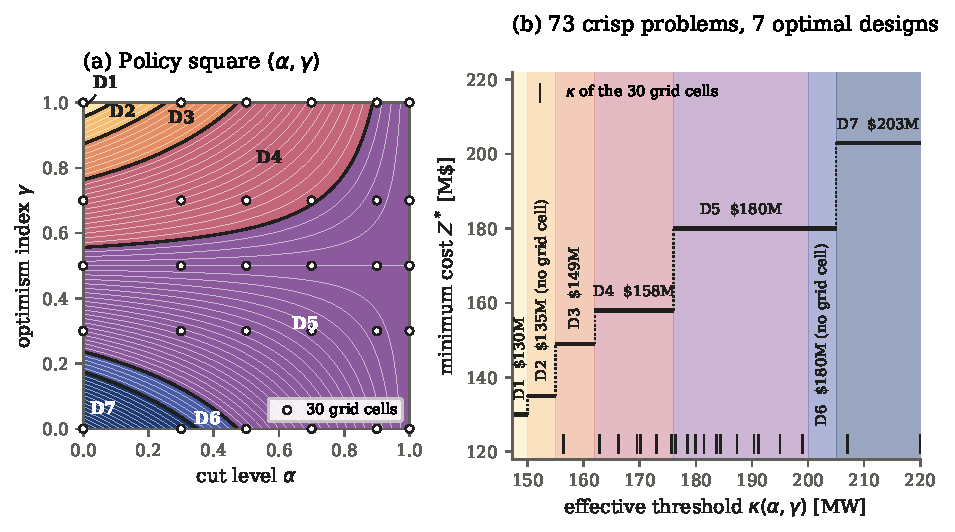
\includegraphics[width=\textwidth]{fig_parametric_partition.pdf}
\caption{\new{Complete parametric solution of the IEEE RTS-79 fleet ($\delta = 0.10$). (a) Optimal design over the policy square. Thin lines are the level curves $\kappa(\alpha,\gamma) = T$ separating the $73$ crisp subproblems; thick lines are the closed-form boundaries $\gamma_T(\alpha)$ of Corollary~\ref{cor:partition} at which the optimal fleet changes; circles are the $30$ cells of the grid (Table~\ref{tab:power_rts_stats}). (b) The same solution against the effective threshold $\kappa$: minimum cost $Z^*$ on each interval $(T-1, T]$, with ticks at the $\kappa$ values of the $30$ grid cells. Designs D1--D7 are numbered by increasing cost; D5 and D6 cost the same and differ in composition. D2 and D6 are optimal on regions that contain no grid cell.}}
\label{fig:parametric}
\end{figure}

\new{Figure~\ref{fig:parametric} shows this solution for the RTS-79 fleet. In panel~(a) the thin lines separate the $73$ crisp subproblems, and the six thick lines are the curves $\gamma_T(\alpha)$ of Equation~\eqref{eq:gamma_T} for $T = 150, 155, 162, 176, 200, 205$, the thresholds at which the optimal fleet changes. Panel~(b) plots the same solution against the single scalar $\kappa$: the minimum cost is a non-decreasing step function of the effective threshold, and each step is one region of panel~(a). The regions are unequal in size. The crisp-optimal fleet D5 ($4\times50$~MW hydro, \$180\,M) is optimal on $61\%$ of the square, and D4 on a further $25\%$.}

\new{The figure also shows what the grid misses. Two of the seven designs are optimal on regions of positive area that contain none of the $30$ grid cells. D2 ($1\times155$~MW coal, \$135\,M, $1.6\%$ of the square) is optimal on the possibility column $\gamma=1$ for $\alpha \in (0.091, 0.254]$, between the grid cells $(0,1)$ and $(0.3,1)$, which prescribe D1 and D3. D6 ($1\times50$~MW hydro and $1\times155$~MW coal, \$180\,M, $3.3\%$) is optimal on the necessity column $\gamma=0$ for $\alpha \in [0.351, 0.474)$, between the grid cells $(0.3,0)$ and $(0.5,0)$, which prescribe D7 and D5. Neither neighbor is optimal there: D5 supplies $200$~MW and cannot meet an effective threshold above $200$~MW, and D7 costs \$23\,M more than D6. Neither design can be recovered from the $30$-cell grid.}

No point of the policy square is left to interpolation. This matters because the design changes
discontinuously at the boundaries, and interpolating between two grid nodes can name a design that is
optimal at neither. The solution was also checked against the grid: each of the $30$
cells was re-solved independently and agreed with the region assigned to it on
cost, reliability and design.

\end{newpart}

\new{Table~\ref{tab:policy_menu} lists the seven designs with their cost, necessity and possibility reliabilities, the share of the square on which each is optimal and the number of grid cells that prescribe it; we call this list the design menu. The menu shows a trade-off that the grid does not. D5, optimal on $61\%$ of the square, and D6, optimal on $3.3\%$ and in no grid cell, have the same cost; D6 has the higher necessity reliability ($0.617$ against $0.506$) and D5 the higher possibility reliability ($0.964$ against $0.953$). A decision maker who gives priority to the necessity of meeting demand would therefore choose D6, which a grid study does not offer.}

\begin{table}[!htbp]
\providecommand{\revtablecolor}{}\revtablecolor
\centering
\caption{Design menu of the IEEE RTS-79 fleet: the seven designs of the complete parametric solution ($\delta=0.10$), with the necessity and possibility reliabilities $R_N$, $R_\Pi$ of each design, the share of the policy square on which it is optimal and the number of the $30$ grid cells that prescribe it.}
\label{tab:policy_menu}
\footnotesize
\begin{tabular}{llrcrrrr}
\hline
Design & Fleet & Cost (M\$) & \shortstack{$T$ range\\on square} & $R_N$ & $R_\Pi$ & Area (\%) & Grid cells\\
\hline
D1 & 1 $\times$ 50 MW Hydro + 1 $\times$ 100 MW Oil & 130 & 148--150 & 0.000 & 0.086 & 0.2 & 1 \\
D2 & 1 $\times$ 155 MW Coal & 135 & 151--155 & 0.000 & 0.244 & 1.6 & 0 \\
D3 & 3 $\times$ 50 MW Hydro + 1 $\times$ 12 MW Oil & 149 & 156--162 & 0.000 & 0.452 & 5.0 & 1 \\
D4 & 2 $\times$ 50 MW Hydro + 1 $\times$ 76 MW Coal & 158 & 163--176 & 0.000 & 0.853 & 25.3 & 6 \\
D5 & 4 $\times$ 50 MW Hydro & 180 & 177--200 & 0.506 & 0.964 & 61.1 & 20 \\
D6 & 1 $\times$ 50 MW Hydro + 1 $\times$ 155 MW Coal & 180 & 201--205 & 0.617 & 0.953 & 3.3 & 0 \\
D7 & 3 $\times$ 50 MW Hydro + 1 $\times$ 76 MW Coal & 203 & 206--220 & 0.951 & 0.978 & 3.5 & 2 \\
\hline
\end{tabular}
\end{table}


\new{Table~\ref{tab:replication} repeats the comparison on the two derived instances.}

\begin{table}[!htbp]
\centering
\caption{The same quantities for the case study and the two literature-derived instances ($30$-cell grid and complete parametric solution of Theorem~\ref{thm:reduction}). A design ``at no grid cell'' is optimal on some region of the policy square but at none of the $30$ grid cells; the last four rows describe the region on which such designs are optimal: its area, the share of it on which the design of the nearest grid cell (closest $\alpha$ and $\gamma$) does not meet the reliability target, the share of the square on which no grid design meets the target, and the largest cost excess over the optimum of the cheapest grid design that meets it. Costs are in the units of each catalog (M\$ for RTS-79).}
\label{tab:replication}
\small
\begin{tabular}{lccc}
\hline
 & IEEE RTS-79 & Fyffe-derived & Pharmaceutical-derived\\
\hline
Design space & $3^{10} = 59{,}049$ & $4^{14} = 2.68\times10^{8}$ & $3^{10} = 59{,}049$\\
Range of $\kappa(\alpha,\gamma)$ & $[147.27,\,220.00]$ & $[36.36,\,66.67]$ & $[30.91,\,51.11]$\\
Integer thresholds (with a feasible design) & 73 (73) & 31 (31) & 22 (20)\\
Distinct optimal designs on the square & 7 & 29 & 20\\
Distinct optimal designs at the grid cells & 5 & 15 & 14\\
Optimal designs at no grid cell & 2 & 14 & 6\\
Minimum cost on the grid & 130--203 & 14--36 & 92--158\\
Grid cells with a feasible design & 30/30 & 30/30 & 29/30\\
\hline
Area optimal at no grid cell (\% of square) & 4.8 & 22.5 & 8.5\\
\quad nearest cell misses target (\% of that area) & 53 & 51 & 65\\
\quad no grid design meets target (\% of square) & 0.0 & 0.0 & 1.6\\
\quad max.\ cost excess of grid design (\%) & 12.8 & 13.3 & 8.4\\
\hline
\end{tabular}
\end{table}


\new{Both findings recur. First, the policy square splits into finitely many regions: $73$, $31$ and $22$ integer thresholds yield $7$, $29$ and $20$ distinct optimal designs, so the complete parametric solution needs a number of integer problems of the same order as the $30$-cell grid. Second, the grid misses part of the solution in every instance, and the part it misses matters. $2$ of $7$, $14$ of $29$ and $6$ of $20$ optimal designs are optimal at no grid cell, and their regions cover $4.8\%$, $22.5\%$ and $8.5\%$ of the square. On $53\%$, $51\%$ and $65\%$ of these regions the design of the nearest grid cell does not meet the reliability target, and the cheapest grid design that does meet it costs up to $12.8\%$, $13.3\%$ and $8.4\%$ more than the optimum. On $1.6\%$ of the square of the Pharmaceutical-derived instance no grid design meets the target, although a design that meets it exists. These figures evaluate the archived designs at each effective threshold and integrate the regions of Corollary~\ref{cor:partition}; no further optimization is involved. A finer grid would reduce them but cannot rule such cases out, whereas the parametric solution covers every point of the square.}


\subsection{The Declared Posture Sets the Design, Its Cost and Its Necessity} \label{sec:posture} \label{sec:sensitivity}

\begin{table}[!htbp]
\centering
\caption{Exact global optimum over the $(\alpha,\gamma)$ grid, IEEE RTS-79-parameterized generation fleet case study. $T$ is the effective integer threshold of Theorem~\ref{thm:reduction} in MW; $R_{\mathrm{sys}}$ is the reliability of the prescribed design under the Hurwicz rule at that cell, and $R_N$, $R_\Pi$ are the graded necessity and possibility reliabilities of the same design (all 30 cells admit feasible certified optima).}
\label{tab:power_rts_stats}
\small
\begin{tabular}{ccrrrrrrr}
\hline
$\alpha$ & $\gamma$ & $T$ & Cost (M\$) & $R_{\mathrm{sys}}$ & $R_N$ & $R_\Pi$ & Nodes & Time (s)\\
\hline
0.0 & 0.0 & 220 & 203 & 0.9509 & 0.951 & 0.978 & 8,366 & 0.00 \\
0.3 & 0.0 & 208 & 203 & 0.9509 & 0.951 & 0.978 & 17,360 & 0.01 \\
0.5 & 0.0 & 199 & 180 & 0.9606 & 0.506 & 0.964 & 1,919 & 0.00 \\
0.7 & 0.0 & 192 & 180 & 0.9606 & 0.506 & 0.964 & 5,573 & 0.00 \\
0.9 & 0.0 & 184 & 180 & 0.9606 & 0.506 & 0.964 & 10,379 & 0.01 \\
1.0 & 0.0 & 180 & 180 & 0.9606 & 0.506 & 0.964 & 12,185 & 0.01 \\
\hline
0.0 & 0.3 & 195 & 180 & 0.9606 & 0.506 & 0.964 & 4,337 & 0.00 \\
0.3 & 0.3 & 191 & 180 & 0.9606 & 0.506 & 0.964 & 5,573 & 0.00 \\
0.5 & 0.3 & 188 & 180 & 0.9606 & 0.506 & 0.964 & 8,525 & 0.01 \\
0.7 & 0.3 & 185 & 180 & 0.9606 & 0.506 & 0.964 & 9,587 & 0.01 \\
0.9 & 0.3 & 182 & 180 & 0.9606 & 0.506 & 0.964 & 12,083 & 0.01 \\
1.0 & 0.3 & 180 & 180 & 0.9606 & 0.506 & 0.964 & 12,185 & 0.01 \\
\hline
0.0 & 0.5 & 180 & 180 & 0.9606 & 0.506 & 0.964 & 12,185 & 0.01 \\
0.3 & 0.5 & 180 & 180 & 0.9606 & 0.506 & 0.964 & 12,185 & 0.01 \\
0.5 & 0.5 & 180 & 180 & 0.9606 & 0.506 & 0.964 & 12,185 & 0.01 \\
0.7 & 0.5 & 180 & 180 & 0.9606 & 0.506 & 0.964 & 12,185 & 0.01 \\
0.9 & 0.5 & 180 & 180 & 0.9606 & 0.506 & 0.964 & 12,185 & 0.01 \\
1.0 & 0.5 & 180 & 180 & 0.9606 & 0.506 & 0.964 & 12,185 & 0.01 \\
\hline
0.0 & 0.7 & 167 & 158 & 0.9605 & 0.000 & 0.853 & 3,458 & 0.00 \\
0.3 & 0.7 & 171 & 158 & 0.9605 & 0.000 & 0.853 & 2,102 & 0.00 \\
0.5 & 0.7 & 173 & 158 & 0.9605 & 0.000 & 0.853 & 1,346 & 0.00 \\
0.7 & 0.7 & 176 & 158 & 0.9605 & 0.000 & 0.853 & 866 & 0.00 \\
0.9 & 0.7 & 179 & 180 & 0.9606 & 0.506 & 0.964 & 12,221 & 0.01 \\
1.0 & 0.7 & 180 & 180 & 0.9606 & 0.506 & 0.964 & 12,185 & 0.01 \\
\hline
0.0 & 1.0 & 148 & 130 & 0.9504 & 0.000 & 0.086 & 329 & 0.00 \\
0.3 & 1.0 & 157 & 149 & 0.9509 & 0.000 & 0.452 & 6,725 & 0.00 \\
0.5 & 1.0 & 163 & 158 & 0.9605 & 0.000 & 0.853 & 5,438 & 0.00 \\
0.7 & 1.0 & 170 & 158 & 0.9605 & 0.000 & 0.853 & 3,362 & 0.00 \\
0.9 & 1.0 & 177 & 180 & 0.9606 & 0.506 & 0.964 & 13,241 & 0.01 \\
1.0 & 1.0 & 180 & 180 & 0.9606 & 0.506 & 0.964 & 12,185 & 0.01 \\
\hline
\end{tabular}
\end{table}


Table~\ref{tab:power_rts_stats} reports the certified optimum in every cell of the grid; every cell admits a feasible fleet. Supplementary Material S6 plots the minimum cost against $\alpha$, one line per $\gamma$. \new{We call $(0,1)$ the optimistic boundary cell: by Proposition~\ref{prop:chance} the column $\gamma=1$ expresses the possibility constraint $\Pi \ge \alpha$ for $\alpha > 0$, and $(0,1)$ is its limit, at which only the supports of capacity and demand have to overlap. The minimum investment ranges from \$130\,M in the optimistic boundary cell $(0.0, 1.0)$, with effective threshold $T = 148$~MW, through \$180\,M in the modal cell $(0.5, 0.5)$, with $T = 180$~MW, to \$203\,M in the necessity cell $(0.0, 0.0)$, with $T = 220$~MW.}

\new{The optimal fleet changes with the declared posture:}
\begin{itemize}
\item In the optimistic boundary cell \new{the rule credits each unit with its upper capacity ($1.1 w_i$) and compares it with the lower demand bound ($162$~MW). The target is met by} one 50~MW hydro unit and one 100~MW oil unit (150~MW modal capacity, $\Rsys = 0.9504$, $R_N = 0.0000$), the remaining bays left empty.
\item In the modal cell the optimal fleet is four 50~MW hydro units (200~MW modal capacity), with $\Rsys = 0.9606$ and $R_N = 0.5056$.
\item In the necessity cell \new{the capacity of the working units must clear the upper demand bound ($198$~MW) even at the lower end of the common spread ($0.9 w_i$). The solver commits} three 50~MW hydro units and one 76~MW coal unit (226~MW modal capacity), with $R_N = \Rsys = 0.9509$.
\end{itemize}
Across the $30$ cells, five of the seven designs of Table~\ref{tab:policy_menu} are optimal: D1, D3, D4, D5 and D7. No 155~MW coal units or 20~MW combustion turbines appear in the optimal designs\new{ of these cells, and oil units appear only in the two most optimistic cells, $(0.0,1.0)$ and $(0.3,1.0)$. The optimal fleets favor the hydro ($p=0.990$) and 76~MW coal ($p=0.980$) units, whose cost per MW ($0.90$ and $0.89$~M\$) is close to that of the larger and less available 100~MW oil and 155~MW coal units ($p=0.960$; $0.85$ and $0.87$~M\$).} Computationally, the solver solves every cell in $\le 0.01$ seconds, exploring between $329$ and $17{,}360$ nodes.

\begin{newpart}
The pair $(\alpha,\gamma)$ specifies a risk posture, and the solver reports, in monetary units, the
rate at which capital expenditure trades against the strength of the guarantee. On the RTS-79 fleet
(Table~\ref{tab:power_rts_stats}) all intervals collapse at $\alpha=1$, and every column gives the
crisp cost of \$180\,M. As $\alpha$ decreases the columns separate. Under the pessimistic rule
($\gamma=0$) the cost rises to \$203\,M ($+12.8\%$); under the optimistic rule ($\gamma=1$) it falls to
\$158\,M at $\alpha=0.7$ and to \$130\,M at $\alpha=0$ ($-27.8\%$). \new{Because the spreads and the threshold
are symmetric, Proposition~\ref{prop:alpha_monotone} and Remark~\ref{rem:monotone_scope} give this pattern
in general: the minimum cost is non-increasing in $\alpha$ for $\gamma<1/2$, which includes the
necessity column, and non-decreasing in $\alpha$ for $\gamma>1/2$.}

The savings come with a weaker guarantee. By Proposition~\ref{prop:chance} the column $\gamma=1$ is, for $\alpha>0$, the possibility
column, so a design prescribed there is one whose success is possible at the stated confidence, not
necessary. The $R_N$ column of Table~\ref{tab:power_rts_stats} measures the difference: the necessity
design costs \$203\,M with $R_N = 0.9509$, the modal design \$180\,M with $R_N = 0.5056$, and on the design menu every design cheaper than \$180\,M has $R_N = 0$. Figure~\ref{fig:insight_policy} shows both quantities
against $\gamma$. For every $\alpha<1$ the minimum cost is non-increasing in $\gamma$, and at $\alpha=0$
it falls from \$203\,M to \$130\,M; the necessity reliability of the prescribed design falls in step,
from $0.95$ at $(0,0)$ to $0.00$ at $(0,1)$. All lines cross at $\gamma=0.5$, where both panels are
independent of $\alpha$. The Fyffe-derived instance, on which more designs are optimal, shows the same trade-off
in finer steps (Supplementary Material S5).

\begin{figure}[!htbp]
\centering
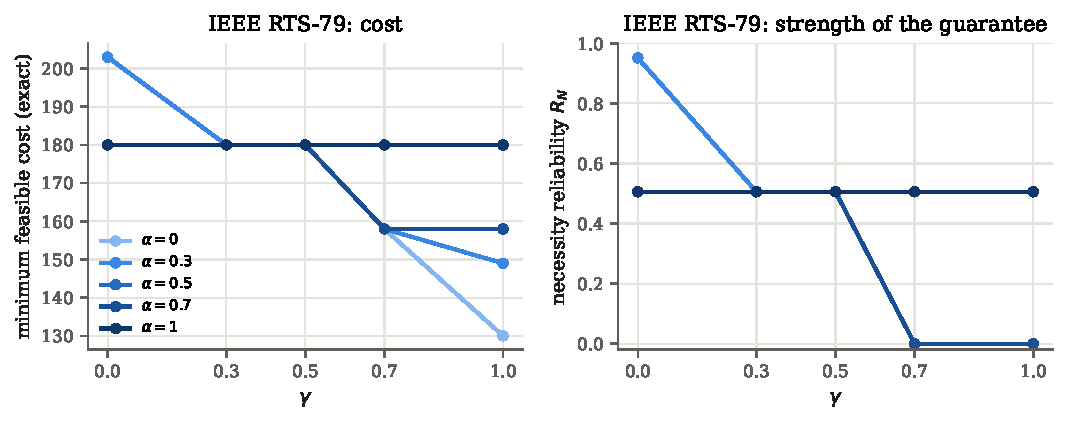
\includegraphics[width=\textwidth]{fig5_policy_effect.pdf}
\caption{\new{Policy effect of the optimism index $\gamma$ on the IEEE RTS-79 fleet. Left: minimum feasible cost. Right: necessity reliability $R_N$ of the design prescribed in each cell. The Hurwicz reliability of every prescribed design clears the target by construction and is therefore not shown; $\alpha=0.9$ is omitted for legibility and reported in Table~\ref{tab:power_rts_stats}. Several lines coincide because few designs are optimal.}}
\label{fig:insight_policy}
\end{figure}

\textbf{Crisp and dual-fuzzy reliability of the same design.} Table~\ref{tab:crisp_vs_fuzzy} compares,
for each design D1--D7 and the same installed units, the classical crisp reliability with the
reliability under the dual-fuzzy rule, and separates the contribution of each fuzzified side. Three
observations follow. First, the crisp model assigns zero reliability to D1--D4, whose modal capacity is
below the modal demand of $180$~MW; in the optimistic boundary cell the same fleets reach $0.950$--$0.970$,
which is why they are prescribed in the optimistic part of the square. Second, part of the effect
appears only when both sides are fuzzy. For D5 and D6, fuzzifying either the capacities or the demand
alone leaves the crisp reliability unchanged in the necessity cell ($0.9606$ and $0.9504$): for D5,
$0.9 \times 200 = 180$~MW still covers the modal demand, and $200$~MW still covers the upper demand of
$198$~MW. Fuzzifying both sides reduces the reliability of both designs to zero, since
$0.9 \times 200 = 180$~MW and $0.9 \times 205 = 184.5$~MW fall short of $198$~MW. D1 and D2 likewise
reach the target in the optimistic boundary cell only when both sides are fuzzified. Third, the necessity design D7 keeps its crisp
reliability ($0.9509$) in the necessity cell under every variant and rises to $0.999$ in the
optimistic boundary cell.

\end{newpart}

\begin{table}[!htbp]
\providecommand{\revtablecolor}{}\revtablecolor
\centering
\caption{Crisp and dual-fuzzy reliability of the same designs (IEEE RTS-79 fleet, designs D1--D7 of Figure~\ref{fig:parametric}). ``Crisp'': modal capacities against the modal demand of $180$~MW. In the necessity cell $(0,0)$ and the optimistic boundary cell $(0,1)$, ``$\tilde{w}$ only'' fuzzifies the capacities and keeps the demand at $180$~MW, ``$\tilde{k}$ only'' fuzzifies the demand and keeps the modal capacities, and ``both'' is the dual-fuzzy model. }
\label{tab:crisp_vs_fuzzy}
\footnotesize
\setlength{\tabcolsep}{4pt}
\begin{tabular}{lrrrrrrrrr}
\hline
 & & & & \multicolumn{3}{c}{Necessity cell $(0,0)$} & \multicolumn{3}{c}{Optimistic boundary cell $(0,1)$}\\
Design & MW & Cost (M\$) & Crisp & $\tilde{w}$ only & $\tilde{k}$ only & both & $\tilde{w}$ only & $\tilde{k}$ only & both\\
\hline
D1 & 150 & 130 & 0 & 0 & 0 & 0 & 0 & 0 & 0.9504 \\
D2 & 155 & 135 & 0 & 0 & 0 & 0 & 0 & 0 & 0.9600 \\
D3 & 162 & 149 & 0 & 0 & 0 & 0 & 0 & 0.9509 & 0.9703 \\
D4 & 176 & 158 & 0 & 0 & 0 & 0 & 0.9605 & 0.9605 & 0.9605 \\
D5 & 200 & 180 & 0.9606 & 0.9606 & 0.9606 & 0 & 0.9606 & 0.9606 & 0.9994 \\
D6 & 205 & 180 & 0.9504 & 0.9504 & 0.9504 & 0 & 0.9504 & 0.9504 & 0.9600 \\
D7 & 226 & 203 & 0.9509 & 0.9509 & 0.9509 & 0.9509 & 0.9797 & 0.9797 & 0.9991 \\
\hline
\end{tabular}
\end{table}


\new{The pattern recurs on the derived instances, whose data are also symmetric: the minimum cost spans $14$--$36$ and $92$--$158$ in the units of their catalogs, is highest on the necessity column $\gamma=0$ and varies with $\alpha$ as on the fleet (Table~\ref{tab:replication}; Supplementary Material S4 and S5). The Pharmaceutical-derived instance adds a case the fleet does not show: in the necessity cell $(0,0)$ no design meets the reliability target, and the two largest integer thresholds have no feasible design.}

\subsection{Ignoring a Source of Imprecision Is Costly} \label{sec:baselines_res}
\begin{newpart}
\begin{table}[!htbp]
\centering
\caption{Model baselines evaluated under the declared dual-fuzzy rule. Each baseline uses the same data and the same posture $(\alpha,\gamma)$ but a simpler model; its design is evaluated at the effective threshold of the dual-fuzzy model. Shares are of the part of the policy square on which some design meets the reliability target. ``Fails'': the baseline design does not meet the target; ``Costlier'': it meets the target at a cost above the optimum; ``Max.\ excess'': largest relative cost excess where it meets the target. Probabilistic counterpart: triangular distributions on the supports of the fuzzy data (Section~\ref{sec:baselines_def}).}
\label{tab:baselines}
\footnotesize
\setlength{\tabcolsep}{4pt}
\begin{tabular}{l rrr rrr rrr}
\hline
 & \multicolumn{3}{c}{IEEE RTS-79} & \multicolumn{3}{c}{Fyffe-derived} & \multicolumn{3}{c}{Pharmaceutical-derived}\\
Baseline & Fails & Costlier & \shortstack{Max.\\excess} & Fails & Costlier & \shortstack{Max.\\excess} & Fails & Costlier & \shortstack{Max.\\excess}\\
 & (\%) & (\%) & (\%) & (\%) & (\%) & (\%) & (\%) & (\%) & (\%)\\
\hline
Crisp (modal data) & 6.8 & 32.1 & 38.5 & 50.0 & 37.6 & 64.3 & 49.9 & 33.4 & 33.7\\
Fuzzy capacities only & 6.8 & 17.1 & 21.5 & 37.7 & 37.6 & 42.9 & 33.5 & 33.4 & 25.0\\
Fuzzy demand only & 6.8 & 16.7 & 21.5 & 33.0 & 27.7 & 21.4 & 30.9 & 30.3 & 16.3\\
Probabilistic counterpart & 6.8 & 93.2 & 49.2 & -- & -- & -- & 33.5 & 66.5 & 44.6\\
\hline
\end{tabular}
\end{table}


Table~\ref{tab:baselines} evaluates the model baselines of Section~\ref{sec:baselines_def} under the
declared rule. The crisp design fails the reliability target on $6.8\%$, $50.0\%$ and $49.9\%$ of the
square of the three instances and, where it meets the target, costs more than the optimum on a further
$32.1\%$, $37.6\%$ and $33.4\%$, by up to $38.5\%$, $64.3\%$ and $33.7\%$. Fuzzifying one side reduces both
effects without removing them: with fuzzy capacities only the design fails on $6.8\%$, $37.7\%$ and
$33.5\%$ of the square, and with fuzzy demand only on $6.8\%$, $33.0\%$ and $30.9\%$. On the RTS-79 fleet
the three model baselines fail on the same region, the part of the necessity side on which the dual
threshold exceeds $200$~MW. No one-sided threshold reaches it, since $k_2/m(\alpha,\gamma)\le 200$~MW and
$\kag\le 198$~MW, and there all three prescribe D5, which supplies $200$~MW. On the derived
instances, whose libraries of optimal designs are finer, the failure regions of the three baselines
differ. Supplementary Material S7 gives these results in full, with the share of the square on which each
baseline design is optimal and its mean cost excess.

The probabilistic counterpart behaves differently. On the RTS-79 fleet, with triangular densities, it
selects four 50~MW hydro units and one 12~MW oil unit at \$194\,M ($R_{\mathrm{prob}}=0.9605$). The
probability that the effective threshold exceeds $200$~MW is $0.034$, and the added oil unit raises the
reliability at the thresholds from $201$ to $212$~MW from zero to $0.941$. This is enough for the average
of Equation~\eqref{eq:rprob} but below the target at each of those thresholds. Under the declared rule the
design therefore fails at every posture whose threshold exceeds $200$~MW ($6.8\%$ of the square), and at
every other posture a cheaper design is optimal: it is optimal at no posture. That alone is not a
defect, since a design chosen by a different criterion need not be optimal at any posture; the frontier
designs of Section~\ref{sec:frontier} share the property. The probabilistic design, however, is not
efficient under that criterion either. It meets crisp adequacy ($R_{\mathrm{modal}}=0.961$), and its
expected necessity reliability, $R_N=0.779$, is below the $0.880$ that the adequacy-constrained
cost--necessity frontier offers at the same budget. With uniform densities on the same supports the
probabilistic design changes to four hydro units and one 20~MW combustion turbine at \$198\,M, so the
prescription depends on a distributional assumption that the data do not fix. On the
Pharmaceutical-derived instance the probabilistic design (cost $133$) is likewise optimal at no posture
and fails the target on $33.5\%$ of the square.
\end{newpart}

\subsection{Menu Designs Need Not Be Efficient in Necessity} \label{sec:frontier}
\begin{newpart}
The design menu (D1--D7) and a cost--necessity trade-off answer different questions. Each menu design minimizes cost subject to
$\Rsys^{\alpha,\gamma}(\mathbf{x}) \ge \Rtarget = 0.95$ in its own cell; it is not selected for its
necessity reliability $R_N$. Its crisp adequacy $R_{\mathrm{modal}}$ (Section~\ref{sec:frontier_model}), the
probability that the working modal capacity reaches $180$~MW, can also differ from the target. D1--D4 install less than $180$~MW ($150$, $155$, $162$ and $176$~MW), so their $R_{\mathrm{modal}}$ is zero.
To relate the menu to the whole catalog we enumerated all $3^{10} = 59{,}049$ designs and solved the
frontier problems of Section~\ref{sec:frontier_model}, Equation~\eqref{eq:biobjective_pareto} and, with
$R_{\mathrm{modal}}(\mathbf{x}) \ge 0.95$, Equation~\eqref{eq:biobjective_pareto_adequate}.
Figure~\ref{fig:true_pareto_frontier} shows both frontiers, and Table~\ref{tab:adequate_frontier} lists the
adequacy-constrained one up to the necessity design D7. The frontier is computed for the case study only.

\begin{figure}[!htbp]
\centering
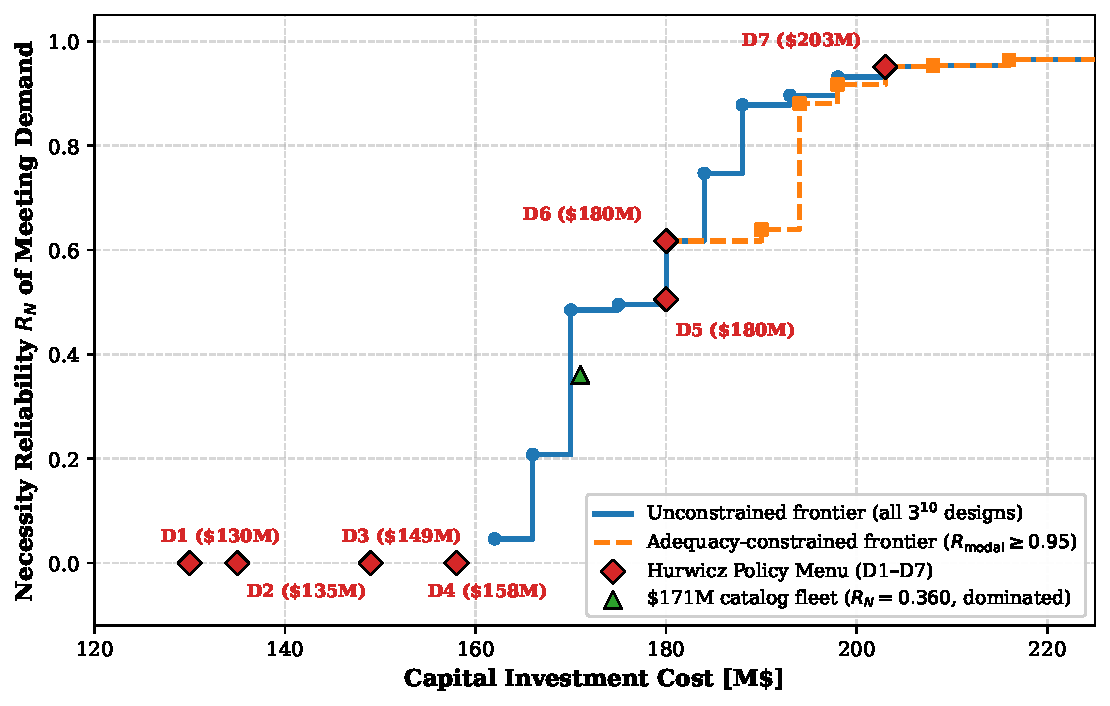
\includegraphics[width=0.85\textwidth]{fig_true_pareto_frontier.pdf}
\caption{\new{Cost--necessity frontiers of the IEEE RTS-79 catalog (exhaustive enumeration of all $3^{10} = 59{,}049$ designs). Solid line: minimum cost subject to $R_N \ge r$ (Equation~\eqref{eq:biobjective_pareto}). Dashed line: the same with crisp adequacy $R_{\mathrm{modal}} \ge 0.95$ (Equation~\eqref{eq:biobjective_pareto_adequate}). Diamonds: design menu D1--D7; D5 and D6 both cost \$180\,M. Triangle: the \$171\,M catalog fleet with the largest $R_N$ ($0.360$), dominated by the \$170\,M frontier design.}}
\label{fig:true_pareto_frontier}
\end{figure}

\begin{table}[!htbp]
\centering
\caption{Adequacy-constrained cost--necessity frontier of the IEEE RTS-79 catalog: designs that minimize cost subject to $R_N(\mathbf{x}) \ge r$ and crisp adequacy $R_{\mathrm{modal}}(\mathbf{x}) \ge 0.95$ at the modal demand of $180$~MW, for every $r$ up to the necessity design D7 (exhaustive enumeration of all $59{,}049$ designs). The last column names the menu design (Table~\ref{tab:policy_menu}) when the frontier design belongs to it.}
\label{tab:adequate_frontier}
\footnotesize
\begin{tabular}{rp{4.6cm}rcccc}
\hline
Cost (M\$) & Fleet & MW & $R_{\mathrm{modal}}$ & $R_N$ & $R_\Pi$ & Menu\\
\hline
180 & 1 $\times$ 50 MW Hydro + 1 $\times$ 155 MW Coal & 205 & 0.9504 & 0.6171 & 0.9528 & D6 \\
190 & 2 $\times$ 50 MW Hydro + 1 $\times$ 76 MW Coal + 1 $\times$ 12 MW Oil + 1 $\times$ 20 MW CT & 208 & 0.9586 & 0.6392 & 0.9663 & -- \\
194 & 1 $\times$ 50 MW Hydro + 1 $\times$ 12 MW Oil + 1 $\times$ 155 MW Coal & 217 & 0.9504 & 0.8804 & 0.9563 & -- \\
198 & 1 $\times$ 50 MW Hydro + 1 $\times$ 20 MW CT + 1 $\times$ 155 MW Coal & 225 & 0.9504 & 0.9171 & 0.9581 & -- \\
203 & 3 $\times$ 50 MW Hydro + 1 $\times$ 76 MW Coal & 226 & 0.9509 & 0.9509 & 0.9782 & D7 \\
\hline
\end{tabular}
\end{table}


Three observations follow.
\begin{enumerate}
\item \emph{Without the adequacy constraint} the frontier contains designs cheaper than \$180\,M with
positive necessity, such as the \$170\,M fleet of two 100~MW oil units ($R_N = 0.4851$). Both oil units
must operate to reach $180$~MW, so its crisp adequacy is $R_{\mathrm{modal}} = 0.960^2 = 0.9216 < 0.95$.
Between \$162\,M and \$203\,M every design of this frontier except the \$180\,M and \$203\,M designs, which
have the composition of D6 and D7, fails crisp adequacy. The two catalog fleets that cost \$171\,M
($1 \times 76$~MW coal $+ 1 \times 100$~MW oil $+ 1 \times 20$~MW combustion turbine, $R_N = 0.3603$; $1 \times 155$~MW coal
$+ 2 \times 20$~MW combustion turbines, $R_N = 0.3110$) are dominated by the \$170\,M fleet.
\item \emph{With the adequacy constraint} no design cheaper than \$180\,M is admissible: the cheapest design
with $R_{\mathrm{modal}} \ge 0.95$ costs \$180\,M, and the frontier starts at D6 ($R_N = 0.6171$). Between D6
and D7 it contains three designs that no Hurwicz cell prescribes (Table~\ref{tab:adequate_frontier}): a planner
bound by adequacy obtains $R_N = 0.6392$ for \$190\,M, $R_N = 0.8804$ for \$194\,M and $R_N = 0.9171$ for \$198\,M, against $0.9509$ for D7
at \$203\,M.
\item \emph{The menu and the frontier differ} because each menu design is the cheapest design at a single
effective threshold $T$; the necessity reliability $R_N$ does not enter that optimization and is reported
for the selected design only.
\end{enumerate}
A decision maker who can relax crisp adequacy may therefore adopt designs such as the \$170\,M fleet,
whereas one bound by it must spend at least \$180\,M and can use Table~\ref{tab:adequate_frontier} to price
necessity levels between those of D6 and D7. The probabilistic design of Section~\ref{sec:baselines_res}
lies below this frontier: at \$194\,M it reaches $R_N=0.779$, against $0.880$.
\end{newpart}


\subsection{The Findings Are Robust to the Spread Model and the Target} \label{sec:robustness} \label{sec:delta_sensitivity}

\begin{newpart}
This subsection checks whether the findings depend on the spread model and on the reliability target,
first through the size and asymmetry of the common spread and the width of the demand forecast. Asymmetry matters for
generation fleets: high ambient temperature reduces the output of combustion turbines through lower air
density and cooling efficiency, whereas low temperature raises it only moderately.

\begin{figure}[!htbp]
\centering
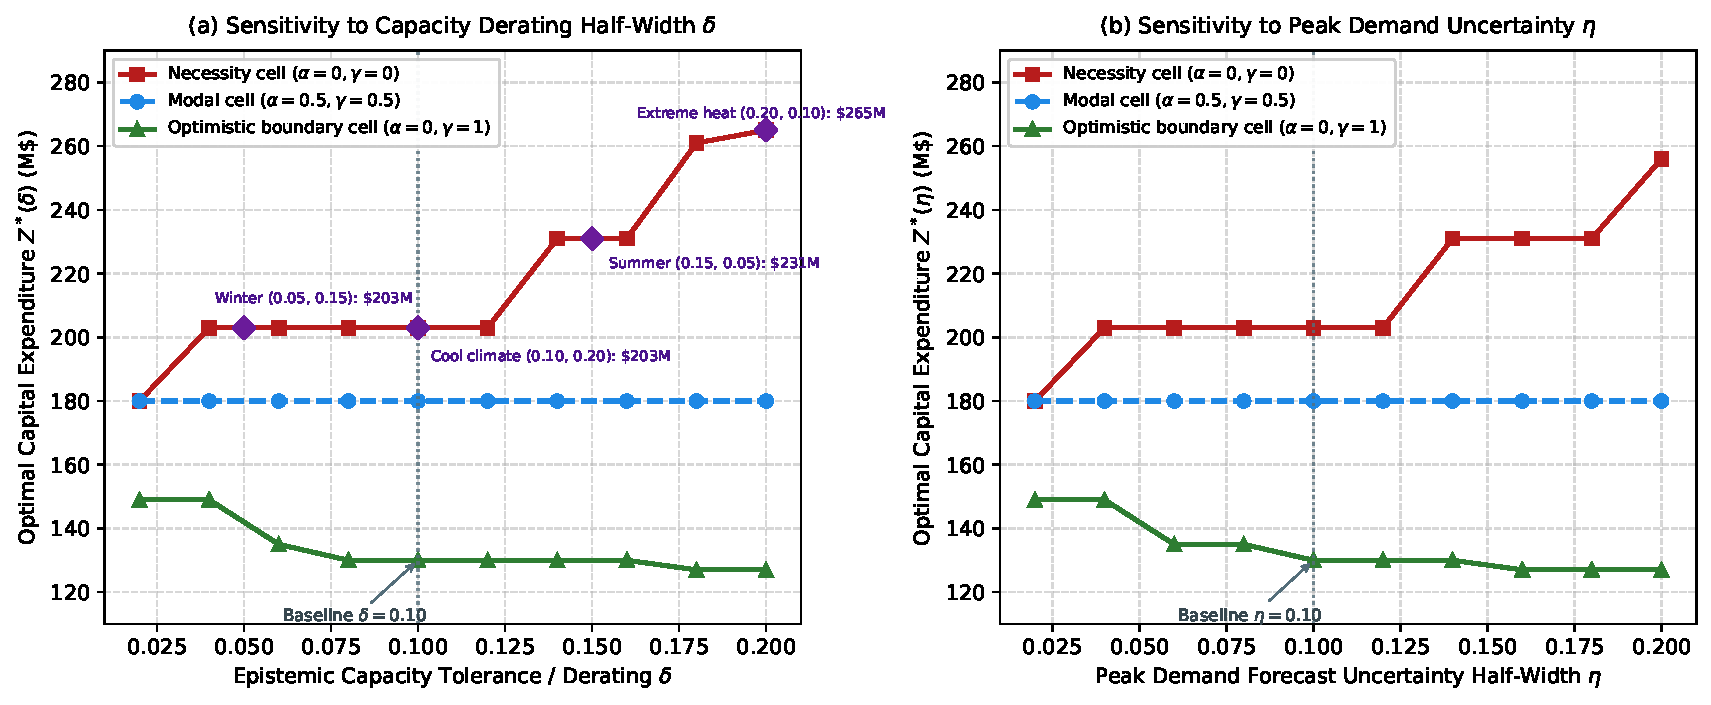
\includegraphics[width=\textwidth]{fig_delta_sensitivity.pdf}
\caption{Sensitivity of optimal capital expenditure to epistemic capacity spread $\delta$ and peak demand forecast uncertainty $\eta$ on the IEEE RTS-79 generation fleet. (a) Sensitivity over the symmetric capacity spread $\delta \in [0.02, 0.20]$; diamonds give the necessity-cell cost under four asymmetric regimes $(\delta_l, \delta_r)$, plotted at $\delta = \delta_l$. (b) Sensitivity to peak demand forecast uncertainty half-width $\eta \in [0.02, 0.20]$.}
\label{fig:delta_sensitivity}
\end{figure}

\textbf{Symmetric spread.} Figure~\ref{fig:delta_sensitivity}(a) traces the optimal cost $Z^*(\delta)$
for $\delta$ from $0.02$ to $0.20$ at ten points, with the demand fixed at
$\tilde{k} = (162, 180, 198)$~MW. Percentages are relative to the modal cost of \$180\,M. Three postures behave differently.
\begin{enumerate}
\item \emph{Necessity $(\alpha,\gamma)=(0,0)$.} The effective threshold
$T = \lceil 198 / (1-\delta) \rceil$ rises from $203$~MW to $248$~MW, and the optimal cost from
\$180\,M to \$265\,M ($+47.2\%$). Under the necessity rule the cost depends only on the downside
spread $\delta_l$.
\item \emph{Modal $(0.5,0.5)$.} The effective threshold stays at $T=180$~MW and the cost at \$180\,M
for every $\delta$. The reason is Equation~\eqref{eq:kappa}: for symmetric spreads the multiplier
$m(\alpha,1/2)$ equals one, and for a symmetric threshold $k^{\alpha}(1/2)=k_2$, so $\kappa=k_2=180$~MW
whatever the value of $\delta$.
\item \emph{Optimistic boundary $(0,1)$.} Wider spreads let the upper capacity bounds $(1+\delta)w_i$ meet the
requirement. At $\delta=0.20$ the effective threshold falls to $T = \lceil 162 / (1+\delta) \rceil =
135$~MW and the cost to \$127\,M ($-29.4\%$). The prescribed design, however, has zero necessity of
meeting demand ($R_N = 0$, $R_\Pi = 0.0751$).
\end{enumerate}

\textbf{Asymmetric spreads.} The markers in Figure~\ref{fig:delta_sensitivity}(a) give the necessity-cell
cost under four stylized seasonal regimes applied to all units: summer, $(\delta_l,\delta_r)=(0.15,0.05)$,
\$231\,M at $T=233$~MW; extreme heat, $(0.20,0.10)$, \$265\,M at $T=248$~MW; winter, $(0.05,0.15)$,
\$203\,M at $T=209$~MW; and cool climate, $(0.10,0.20)$, \$203\,M at $T=220$~MW, as for the symmetric
$10\%$ spread, because the upside does not enter the necessity rule. Under every asymmetric regime the modal cell $(0.5,0.5)$ moves as well, because $m(0.5,0.5) = 1 + (\delta_r - \delta_l)/4 \ne 1$: its threshold is $T = 185$~MW (\$180\,M) for summer and extreme heat and $T = 176$~MW (\$158\,M) for winter and cool climate. Asymmetric spreads need no additional computation: Theorem~\ref{thm:reduction} allows $\delta_l \ne \delta_r$, so every
regime is solved through Equation~\eqref{eq:kappa} with the same certificate.

\textbf{Demand uncertainty.} Figure~\ref{fig:delta_sensitivity}(b) varies the half-width $\eta$ of the
demand forecast $\tilde{k} = (180(1-\eta), 180, 180(1+\eta))$ from $0.02$ to $0.20$. Under the
necessity rule the cost rises from \$180\,M to \$256\,M; in the optimistic boundary cell it falls to
\$127\,M.
\end{newpart}

\new{\textbf{Reliability target.} At $\Rtarget=0.95$ the cost-minimizing fleets of the optimistic boundary, modal and necessity cells are series arrangements at their threshold: the loss of any single unit drops the working capacity below $T$. Repeating the optimization for $\Rtarget\in\{0.90,0.91,\dots,0.99\}$ at the thresholds of these three cells (Supplementary Material S6), a fleet that still reaches $T$ after the loss of its largest unit becomes optimal at $\Rtarget=0.97$ in the modal cell (\$212\,M) and at $0.98$ in the other two (\$180\,M and \$266\,M). These breakpoints are properties of this catalog and target range, not general rules.}

\begin{newpart}
\textbf{Unit-specific spreads.} Theorem~\ref{thm:reduction} requires the same proportional spread for every unit. RTS-79
gives the available capacity of its hydro units as $100\%$ of the $50$~MW rating in two quarters and $90\%$
in the other two (its Table~6), so the hydro capacity is $(45,50,50)$~MW, $(\delta_l,\delta_r)=(0.10,0)$;
for the thermal units we assume $(0.15,0.05)$ for the combustion turbines and $(0.05,0.02)$ for the
steam units, which encode the qualitative effect of ambient temperature rather than measured derating
curves. With heterogeneous spreads the reduction fails, and each of the $30$ cells is solved by the
unreduced exact search; all complete within $600$~s, the slowest in $234$~s. The optimal fleet changes in
$7$ of the $30$ cells and its cost in $6$, in both directions. On the necessity side the common spread
over-invests: at $(0.3,0)$ the unit-specific optimum costs \$180\,M instead of \$203\,M, a saving due to
the thermal spreads alone. On the possibility side it under-invests: in five cells the unit-specific
model needs \$9--22\,M more, mainly because the common spread credits a hydro unit with up to $55$~MW.
A single common-spread control $(0.06,0.02)$ reproduces $5$ of the $7$ changes, and varying the assumed
thermal and hydro spreads leaves six of the seven changed cells unchanged; cell $(0.3,0.7)$ is the least
robust. Supplementary Material S6 gives the cell-by-cell results, the decomposition into thermal and
hydro effects and the sensitivity runs.

\textbf{Relation to Theorem~\ref{thm:reduction}.} At these spreads every unit-specific optimum is the crisp optimum of some
integer threshold, that is, a member of the library of Section~\ref{sec:parametric}. That coincidence is
not general: under the perturbed thermal spreads the optimum at $(0.3,0.7)$ is a \$171\,M fleet of one
155~MW coal unit and two 20~MW combustion turbines, which is the crisp optimum of no integer threshold;
an exhaustive enumeration in exact rational arithmetic confirms both its optimality and its absence from
the library. Heterogeneous spreads can therefore select a design that no single effective threshold
would, and only the unreduced search finds it.

Across these variants the declared posture keeps changing the prescribed fleet and its cost, in both
directions, which is the finding of Section~\ref{sec:posture}.
\end{newpart}

\begin{newpart}
\subsection{Certification Scales to $n=20$} \label{sec:scaling}

We solved a family of synthetic catalogs with three
choices per subsystem at $n \in \{8,10,\dots,20\}$ under three demand profiles (\emph{screening},
\emph{design} and \emph{stringent}, with loose, moderate and tight thresholds), $21$ instances in total,
with the reduction of Theorem~\ref{thm:reduction}, a compiled recursion and a $600$~s budget per instance. All $21$
completed with a certificate.

\begin{table}[!htbp]
\centering
\caption{Certified exact solution of the synthetic scaling family ($3$ choices per subsystem, design
profile shown; $T$ is the effective integer threshold of Theorem~\ref{thm:reduction}). ``Leaves'' counts complete
designs actually evaluated. The instances $n=8$ and $10$ (solved in at most $0.012$~s) are omitted.}
\label{tab:scaling}
\small
\begin{tabular}{rrrrrrr}
\hline
$n$ & Search space $3^n$ & $T$ & Time (s) & Nodes & Leaves & Optimal cost\\
\hline
12 & $5.31\times10^{5}$ & 60 & 0.03 & $5.66\times10^{4}$ & 7 & 63\\
14 & $4.78\times10^{6}$ & 66 & 0.27 & $6.09\times10^{5}$ & 35 & 77\\
16 & $4.30\times10^{7}$ & 78 & 6.20 & $1.49\times10^{7}$ & 29 & 99\\
18 & $3.87\times10^{8}$ & 81 & 30.41 & $6.23\times10^{7}$ & 47 & 111\\
20 & $3.49\times10^{9}$ & 100 & 459.24 & $8.35\times10^{8}$ & 89 & 117\\
\hline
\end{tabular}
\end{table}

Table~\ref{tab:scaling} reports the design profile, the hardest of the three. Two quantities describe
the pruning. The node count measures the work of the search, including the internal nodes of partial
designs: at $n=20$ the solver expands $8.35\times10^{8}$ nodes of a full ternary tree of
$(3^{21}-1)/2 = 5.23\times10^{9}$ nodes, or $15.96\%$. This count is comparable with the size of the
tree, not with $3^{20}$, which counts complete designs. The leaf count is the number of complete candidate designs reaching depth $n$ whose exact reliability is evaluated: $89$ of $3.49\times10^{9}$. The admissible bounds thus discard almost every complete design at interior levels before constructing it.

\textbf{Ablation.} Progress from $n=14$ to $n=20$ combines an algorithmic change and a larger budget.
Table~\ref{tab:ablation} gives the frontier of each regime.

\begin{table}[!htbp]
\centering
\caption{Largest instance certified under each regime (design profile, $12$~s iso-budget unless stated).}
\label{tab:ablation}
\small
\begin{tabular}{lll}
\hline
Regime & Configuration & Frontier\\
\hline
1 & Interpreted backend, unreduced threshold, $12$~s & $n = 12$ ($n=14$ times out)\\
2 & Compiled backend, reduced threshold, $12$~s & $n = 16$ ($6.20$~s; $n=18$ times out)\\
3 & Compiled backend, reduced threshold, $600$~s & $n = 20$ ($459.24$~s; $0$ censored)\\
\hline
\end{tabular}
\end{table}

Regimes~1 and~2 share the budget and differ only in formulation and implementation: the certified
frontier moves from $n=12$ to $n=16$. To separate the reduction from the compiler, we re-solved the
$n=14$ design instance with the same compiled backend but without the reduction, that is, against a
threshold obtained by scaling the continuous fuzzy endpoints into integers (scale factor $10^4$, giving
an unreduced threshold of $16{,}767$ against $T=66$ for the reduced model). It required $60.69$~s,
against $0.268$~s for the reduced formulation, a factor of $226.8$. The factor is close to the ratio of
the thresholds ($16{,}767 / 66 \approx 254$), as expected, because the convolution table is
proportional to the integer threshold. The gain from Theorem~\ref{thm:reduction} therefore comes from replacing a finely
scaled threshold by the modal integer threshold, without any discretization of the state. Regime~3
shows that a larger budget extends certification to $n = 20$.

The reduction does not change the solutions. Across all $12$ instances up to $n=14$, the reduced and
unreduced formulations agreed on cost, reliability and design. Above $n=14$ the unreduced solve
exceeds the budget and returns no verdict, so no agreement is claimed there. Neither the bounds nor the
reduction removes the exponential worst case; on the instances studied, certified optima are obtained
within the reported budgets, and every cell of the RTS-79 fleet solves in at most $0.01$~s.

\subsection{Certification Matters at the Secondary Objective} \label{sec:baseline}

Because metaheuristics are the usual method in this literature, we compared the exact solver with a
genetic algorithm (population $\max(60, 12n)$, ternary tournament selection, uniform crossover, per-gene mutation with rate $1.5/n$, elitism of two individuals, and feasibility-first lexicographic comparison) across $17$ instances (Table~\ref{tab:baseline}): the RTS-79 fleet, the Fyffe-derived instance, and the $15$ non-trivial synthetic scaling instances ($n \in \{12, 14, 16, 18, 20\}$ under all three demand profiles, drawn from the 21-instance family of Section~\ref{sec:scaling}; the small instances $n \in \{8, 10\}$ solve in at most $0.012$~s and were excluded as trivial for heuristic benchmarking).

A fair comparison requires matched computational effort. A heuristic that stops at its own stagnation
rule after a few seconds, while the exact solver runs for minutes, uses only a fraction of the budget.
We therefore made the heuristic restart on stagnation so that it uses its whole budget, and ran two
protocols. Protocol~A gives the heuristic the same wall-clock time the exact solver used on that
instance, with a minimum of $5$~s. Protocol~B gives it $1{,}000{,}000$ objective evaluations on the two
instances where the outcome differed; because the heuristic is interpreted and the exact solver
compiled, wall-clock matching favors the exact solver, whereas an evaluation budget does not. In both
protocols the heuristic's incumbent is then refined by an equal-cost local search (single-subsystem
substitutions of identical cost and pairwise swaps whose cost changes cancel), the refinement a
practitioner would apply when the secondary objective is reliability.

After this refinement the heuristic matched the certified optimum on both objectives in all five seeds
on $16$ of the $17$ instances. The exception is the largest instance, $n=20$ under the design profile,
where all five seeds reached the minimum cost of $117$ but one seed under Protocol~A, and two under
Protocol~B, settled on a design whose reliability is $0.9035$ against the certified $0.9112$, a
shortfall of $7.7\times10^{-3}$. The refinement did not close the gap: it terminated after $16$ to $23$
evaluations without improvement, because the better design cannot be reached from the incumbent through
cost-preserving moves. At $n=14$ under the same profile, one seed missed the secondary optimum before
refinement, and the refinement recovered it.

\begin{table}[!htbp]
\centering
\caption{Genetic-algorithm baseline against the certified optimum, five seeds per instance.
``Cost'' counts seeds reaching the minimum cost; ``Secondary'' counts those also reaching the
maximum-reliability design at that cost.}
\label{tab:baseline}
\small
\begin{tabular}{llcccc}
\hline
Instance & Protocol & Budget & Cost & Secondary & Shortfall\\
\hline
\new{$15$ other} instances & A & matched wall-clock & $5/5$ & $5/5$ & ---\\
$n=14$ design & A & $5.0$~s & $5/5$ & $4/5 \to 5/5$ after refinement & $0$\\
$n=14$ design & B & $10^{6}$ evaluations & $5/5$ & $5/5$ & $0$\\
$n=20$ design & A & $365.2$~s$^a$, $2.50\times10^{6}$ eval. & $5/5$ & $4/5$ & $7.7\times10^{-3}$\\
$n=20$ design & B & $10^{6}$ evaluations, $146$~s & $5/5$ & $3/5$ & $7.7\times10^{-3}$\\
\hline
\multicolumn{6}{l}{\footnotesize $^a$ The exact runtime for $n=20$ is recorded as $365.2$~s under Protocol~A and $459.2$~s under the scaling campaign;}\\
\multicolumn{6}{l}{\footnotesize \phantom{$^a$} the difference reflects separate runs with different profiling overhead on the host.}\\
\hline
\end{tabular}
\end{table}

Without a certificate, nothing in the heuristic's output indicates that a more reliable design exists
at the same cost.
\end{newpart}


\section{Discussion} \label{sec:discussion}

\subsection{Managerial Implications} \label{sec:managerial} \label{sec:policy_map} \label{sec:selecting}
\begin{newpart}
Section~\ref{sec:posture} showed that the pair $(\alpha,\gamma)$ fixes, in monetary units, the rate at
which capital expenditure trades against the strength of the guarantee.
For the choice of posture, the square divides into three zones. Low $\alpha$ with low $\gamma$
compares the worst-case capacity with the worst-case threshold on the widest cut. By Proposition~\ref{prop:chance} the
cell $(\alpha,0)$ demands necessity $1-\alpha$, so conservatism increases as $\alpha$ decreases. This
zone gives the highest cost (\$203\,M) and suits safety-critical infrastructure in which shortfalls
carry severe penalties. Low $\alpha$ with high $\gamma$ approaches the optimistic boundary cell, with the lowest cost
(\$130\,M) and zero necessity of meeting demand; it suits non-critical deployments in which
occasional shortfalls are tolerable. As $\alpha \to 1$ every interval collapses to its modal value,
$\gamma$ loses its effect, and all columns converge on the crisp design (\$180\,M). Intermediate pairs
represent negotiated compromises, for which the solver gives the marginal cost of each step towards
more conservatism.

\end{newpart}

\begin{newpart}
The pair $(\alpha,\gamma)$ need not be chosen as two free numbers. The results of
Sections~\ref{sec:family} and~\ref{sec:parametric} give three ways of fixing it, in decreasing order of
what they require from the decision maker.

\textbf{(i) A prescribed necessity level.} When a regulation, a contract or an internal standard
requires demand to be met with necessity at least $\lambda$, Proposition~\ref{prop:chance} fixes the cell
$(1-\lambda,0)$, and no optimism index has to be elicited. A requirement stated as a possibility or
credibility level fixes a cell in the same way (Table~\ref{tab:nesting}).

\textbf{(ii) A design menu.} Without such a requirement, the decision maker can choose among designs
instead of parameters. The complete parametric solution is a finite menu: on the RTS-79 fleet it
contains the seven designs of Table~\ref{tab:policy_menu}, each with its cost, its necessity and
possibility reliabilities and the share of the square on which it is optimal. Choosing a design fixes
the set of postures consistent with that choice. A capital budget $\bar{Z}$ is a special case: the menu gives
the design with the largest necessity reliability among those costing at most $\bar{Z}$. With $\bar{Z}$ set to \$150\,M no
affordable design has a positive necessity of meeting demand, \$180\,M buys $R_N = 0.617$ (D6, the better of the two \$180\,M designs) and
\$203\,M buys $R_N = 0.951$; under crisp adequacy the catalog offers $R_N = 0.880$ for \$194\,M and $0.917$ for \$198\,M (Table~\ref{tab:adequate_frontier}), designs that are not on the menu. The menu contains the designs that are optimal in some cell of the Hurwicz square;
it is not the set of designs that minimize cost subject to a necessity requirement, which is a different
optimization problem (Section~\ref{sec:frontier}).

\textbf{(iii) An elicited optimism index.} If an interior value of $\gamma$ is wanted, it follows from
Equation~\eqref{eq:hurwicz_w} once the decision maker states a certainty equivalent $C^*$ for an interval
$[C_{\min},C_{\max}]$: $\gamma = (C^*-C_{\min})/(C_{\max}-C_{\min})$. Because the optimal design is
piecewise constant in $\gamma$, the elicited value matters only through the region it falls in, and
Corollary~\ref{cor:partition} gives that region exactly. At fixed $\alpha<1$, $\kappa$ decreases in $\gamma$, so the
optimal design is unchanged for $\gamma \in [0,1]$ with $\gamma_{T_{\max}}(\alpha) \le \gamma < \gamma_{T_{\min}-1}(\alpha)$,
where $T_{\min}$ and $T_{\max}$ are the smallest and largest effective thresholds of the region. At
$\alpha=0.5$, for example, the modal design D5 is optimal for every $\gamma<0.612$, so an elicitation
error below that value does not change the prescription; at $\alpha=0$ the necessity design D7 is
optimal only for $\gamma<0.175$. The attitude of an individual manager is a weaker basis for
safety-critical infrastructure than a prescribed necessity level, and we regard (iii) as a fallback.
The script that produces the menu, the budget inversion and the intervals is listed in Supplementary
Material S2.
\end{newpart}

\new{\textbf{What the baselines imply.} A planner who solves the crisp model, or fuzzifies one side only, commits without stating it to a design that is optimal for some postures and not for others; Table~\ref{tab:baselines} shows how large the part of the square is on which that design fails the target, and Section~\ref{sec:parametric} shows the same for a grid study. The probabilistic counterpart is not a neutral alternative: it needs densities that expert-based data do not fix, and on the case study its prescription changed with the density. Declaring the posture and solving over the whole square makes the commitment explicit and its consequences measurable.}

\begin{newpart}
\subsection{Relation to Other Uncertainty Frameworks} \label{sec:frameworks}
A probabilistic model needs distributions for the capacities and the threshold, and fitting them needs
frequency data; when targets and derating bands come from regulations and expert judgement, such data
are often unavailable \citep{Zio2009}. The probabilistic counterpart of Section~\ref{sec:baselines_res}
illustrates the consequence: with the same supports, the prescribed design depends on the assumed
density. Liu's credibility measure \citep{Liu2002} is self-dual, which possibility and necessity
individually are not. By Corollary~\ref{cor:credibility} a credibility chance constraint on the success condition is a cell
of the square, so the designs it prescribes are among those of the parametric solution; a requirement
on the expected credibility reliability averages the two extreme columns and, like the cost--necessity
frontier, is not a cell. The plain worst case over the supports of the fuzzy data is the cell
$(0,0)$. Robust formulations that limit how many quantities may deviate at once \citep{BertsimasSim2004},
or that minimize the maximum regret over interval data \citep{FeizollahiModarres2012}, are not points of
the square and are left to future work (Section~\ref{sec:limitations}). The uncertainty theory of \citet{Liu2015} replaces the possibilistic set
functions with an axiomatic uncertain measure and is a different formalism. Supplementary Material S4
solves the Fyffe and Pharmaceutical catalogs with the uncertain-measure oracle of
\citet{WeiShiZhang2025a} in place of the possibilistic one: on the Pharmaceutical catalog the uncertain
measure declares the instance infeasible, and on the Fyffe catalog it selects a different design.
Supplementary Material S3 records the verification of that oracle against its published worked example.
Possibilistic evaluation reduces to comparisons of $\alpha$-cut endpoints, which is what allows the exact
solver to propagate capped capacity distributions and to compute admissible bounds.
\end{newpart}

\subsection{Study Limitations} \label{sec:limitations}

The following structural limitations define the current scope:
\begin{enumerate}
\begin{newpart}
    \item Exactness does not imply unlimited scalability. Certified solution is demonstrated up to $n=20$ with three choices per subsystem; beyond the sizes actually solved we make no claim, and larger deployments may require decomposition or hybridization with metaheuristic surrogates.
  \item The dimensional reduction of Theorem~\ref{thm:reduction} requires capacity spreads that are proportional and common to all components. Asymmetric spreads are covered ($\delta_l$ and $\delta_r$ need not be equal), but component-specific spreads reintroduce subset dependence in the aggregate, so the parametric partition does not collapse onto a single scalar. As shown in Section~\ref{sec:robustness}, \new{the exact branch-and-bound engine still solves the unit-specific problem, cell by cell and without the closed-form reduction, at a markedly higher computational cost; at the base spreads of that case study every unit-specific optimum coincides with a crisp-threshold optimum, but under nearby spread values a fleet that is optimal for no integer threshold is selected, so the crisp family does not in general contain the unit-specific optimum.} Higher-order fuzzy sets such as Z-numbers or intuitionistic fuzzy sets are not covered \citep{MANECKSHAW2026129956}.
  \item \new{The uncertainty-theory baseline in Supplementary Material Section~S4 rests on a translation between formalisms: component reliabilities are read as uncertain state measures and capacity TFNs as zigzag uncertain variables. The translation is natural but not canonical, and imposing the same nominal confidence level on an uncertain measure and on a possibilistic reliability is a convention adopted for comparability. The experiment therefore shows that the choice of calculus changes the prescription; it does not adjudicate between the calculi.}
  \item The chance-constraint correspondence of Proposition~\ref{prop:chance} is a statement about the success condition of a subset, not about the reliability of a design. A necessity requirement and the cell it maps to accept the same subsets, yet the expected necessity reliability $R_N$ weights each subset by its necessity and can differ from the reliability at that cell; Proposition~\ref{prop:decomposition}, with the equivalence that follows it, is the bridge we establish between the two levels.
\end{newpart}

  \item \new{The cost--necessity frontier of Section~\ref{sec:frontier_model} and the probabilistic counterpart average the reliability over many effective thresholds, so the single-threshold bounds of the exact solver do not apply to them; both were computed by exhaustive enumeration, which limits them to the catalogs with $3^{10}$ designs.}
  \item \new{The model baselines are evaluated under the declared dual-fuzzy rule. The probabilistic counterpart assumes a common derating factor, independence between derating, demand and unit states, and densities on the supports of the fuzzy data; other dependence structures or densities would select other designs.}
  \item \new{The model baselines do not include robust counterparts. A budgeted-uncertainty formulation \citep{BertsimasSim2004} lets at most $\Gamma$ capacities fall to their lower bounds; the worst case then depends on which units a subset contains, not only on its total capacity, so the formulation is not a cell of the square and the single-threshold reduction of Theorem~\ref{thm:reduction} does not apply to it. A min--max regret design \citep{FeizollahiModarres2012} requires the optimum of every scenario. Neither was computed, so the extent to which dual-fuzzy and robust designs differ is not quantified here.}
  \item Statistical independence of components is a structural assumption. Shared-load and cascading failure dependencies \citep{WU2025110678} are not modeled.
  \item \new{The IEEE RTS-79 fleet takes its capacities and availabilities from the published test system, but its capital costs are an assumption of this study (Section~\ref{sec:rts_benchmark}). The two literature-derived instances are adaptations, not the original problems: in the Fyffe-derived instance capacities were reinterpreted from physical weight and parallel redundancy was removed, and most values of the Pharmaceutical-derived instance are synthetic (Section~\ref{sec:rts_benchmark}); their costs are therefore not comparable with published solutions. Calibrated benchmarks from other industrial domains, such as municipal pumping networks and data-center power systems, are a natural subject for future empirical studies.}
  \item \new{The results depend on the shapes of the membership functions, which should be elicited and reviewed with domain experts before industrial use.}
\end{enumerate}

\section{Conclusion} \label{sec:conclusion}
\begin{newpart}
When the component capacities and the demand threshold of a weighted $k$-out-of-$n$:G system are both
imprecise, the success condition needs a comparison rule. This paper declares that rule as a Hurwicz
comparison on $\alpha$-cuts and draws three conclusions, one for each research question.

First (\rqref{rq:rule}), the rule contains the readings that the literature uses separately: the crisp model, the
interval worst and best cases, and the necessity-, possibility- and credibility-based chance constraints
are points of one policy square, and averaging its extreme columns over the cut level gives the
expected necessity and possibility reliabilities.

Second (\rqref{rq:parametric}), under common proportional capacity spreads the square acts on the design problem through
one effective integer threshold, so the optimal design is known at every point of the square from a
number of integer problems of the same order as a $30$-cell grid. The grid itself misses part of the solution
on all three instances studied, and where it does, the design of the nearest grid cell fails the target
on more than half of the area. Simpler models with the same data are costly as well: the crisp design
fails the target on up to half of the square and costs up to $64\%$ more than the optimum elsewhere,
one-sided fuzzy models fail on up to $38\%$, and a probabilistic counterpart, computed on two of the
instances, selects designs that are optimal at no posture, change with the assumed density and, on the
case study, are dominated in expected necessity. Designs prescribed at a reliability
target need not be efficient in necessity; on the case study the cost--necessity frontier contains
designs that no cell prescribes.

Third (\rqref{rq:solver}), the two-phase branch-and-bound solver certifies every instance up to $n=20$; a
budget-matched genetic algorithm reproduces the minimum cost throughout but, at the largest instance,
settles in some seeds on an equal-cost design with lower reliability.

Four directions follow. Component-specific or additive spreads break the factorization of Theorem~\ref{thm:reduction},
and identifying the weakest condition under which a reduction of this kind survives would extend the
complete solution to a wider class of fuzzifications. An exact method for the cost--necessity frontier,
which averages over many thresholds, would remove the enumeration used here. \new{A quantitative comparison with budgeted-uncertainty and min--max regret designs, which lie outside the square, would show when a declared posture and a robustness budget lead to the same fleet.} Dependence between
components, such as shared load and cascading failure, remains outside the present model and is the
more consequential restriction for infrastructure applications.
\end{newpart}

\section*{Statements and Declarations}

\bmhead{Competing interests}
The author declares no known competing financial or non-financial interests that are directly or
indirectly related to the work reported in this paper.

\bmhead{Funding}
This research received no specific grant from any funding agency in the public, commercial or
not-for-profit sectors.

\bmhead{Author contributions}
Kadir Sar\i kaya: Conceptualization, Methodology, Formal analysis, Software, Validation,
Investigation, Data curation, Writing -- original draft, Writing -- review and editing,
Visualization.

\bmhead{Data availability}
All source code, benchmark data and computational artifacts required to reproduce the reported results
are publicly available at \href{https://github.com/k-sarikaya/FuzzyWeighted}{https://github.com/k-sarikaya/FuzzyWeighted}.
The case study and the two derived instances are built from published sources (IEEE RTS-79, \citealp{IEEERTS1979};
Fyffe problem, \citealp{Fyffe1968}; Pharmaceutical Plant, \citealp{Garg2013}); no proprietary or third-party restricted data were used. The
deterministic pipeline, the script producing each reported result, the verification checks and the
computational environment are documented in Supplementary Material S2.

\bmhead{Use of generative AI}
During the preparation of this work the author used generative AI tools to assist with language
editing. After using these tools the author
reviewed and edited the content as needed and takes full responsibility for the content of the
published article.

\bibliography{sn-bibliography}% common bib file
\end{document}
